% ============================================================
%  第十章  软件使用说明
% ============================================================
\section{软件使用说明}

本章说明软件“怎么用”。先介绍界面风格与通用操作，再按页面给出标注了编号的界面截图、操作步骤与区域用途说明，最后把常用操作串成三条典型流程，并汇总常见问题。截图取自 V1.0 实际运行界面（默认深色主题，1600$\times$1000 视口）。

\subsection{快速上手}

\subsubsection{启动与入口}

软件有两个入口（表~\ref{tab:use_entry}）。日常使用推荐第一种，双击或执行一条命令即可同时启动两个模块并打开桌面窗口。

\begin{table}[H]
\centering
\caption{启动方式与访问地址}
\label{tab:use_entry}
\small
\begin{tabularx}{\linewidth}{@{}>{\ttfamily}p{4.4cm}>{\raggedright\arraybackslash}X@{}}
\toprule
命令 & 说明 \\
\midrule
python main.py & 桌面窗口，两个模块同时运行（推荐） \\
python main.py --headless & 不弹窗口，用浏览器访问两个地址 \\
python main.py recon & 只启动轨迹重建与分析（5000） \\
python main.py recog & 只启动无人机检测（5001） \\
\bottomrule
\end{tabularx}
\end{table}

启动成功后，浏览器访问 \url{http://127.0.0.1:5000} 进入轨迹重建与分析，访问 \url{http://127.0.0.1:5001} 进入无人机检测；在 5000 页面点击导航栏右侧的“识别”可直接跳转到检测模块。

\subsubsection{首次使用要做的三件事}

\begin{enumerate}
  \item \term{准备数据}：\file{data/fact/} 目录下至少有一个平台的轨迹文件（如 \file{visible.npz}）。软件自带示例数据，首次启动即可看到轨迹。
  \item \term{准备检测模型}：\file{models/yolo/detect.pt} 为检测权重；未放置时检测页仍可打开，但无法开始检测。
  \item \term{配置 AI 密钥（可选）}：编辑 \file{config.json} 的 \code{ai} 段，填入可用的接口地址、密钥与模型名，才能使用“AI 策略”；不配置不影响其它功能。
\end{enumerate}

\subsection{界面总览与通用操作}

\subsubsection{界面风格}

界面采用统一的设计语言，由 \file{templates/frontend/static/css/main.css} 中的 CSS 变量驱动：

\begin{itemize}
  \item \term{导航栏}：固定在顶部，左侧为品牌与五个主功能入口，右侧为“识别 / 帮助 / 设置”三个辅助入口；当前页高亮。
  \item \term{面板}：半透明毛玻璃背景、1 px 描边、8 px 圆角；面板标题左侧配线性图标。
  \item \term{配色}：深色主题以深蓝灰为底，主色为蓝色，五个平台各有专属颜色（可见光珊瑚红、红外青绿、雷达黄、自选橙、综合白）。
  \item \term{图形语言}：全部图标为几何风格 SVG，不使用 emoji；数值统一使用等宽字体，便于对齐比较。
  \item \term{双主题}：深色/浅色主题通过 \code{data-theme} 属性切换，所有颜色由变量定义，切换时无需刷新页面。
\end{itemize}

\subsubsection{界面结构}

两个模块界面风格一致：顶部导航栏、中间内容区、右下角浮层提示。以总览页为例，界面由五个部分组成（图~\ref{fig:use_dashboard}）。

\begin{figure}[H]
\centering
\begin{tikzpicture}
\node[inner sep=0, anchor=south west] (im) at (0,0)
  {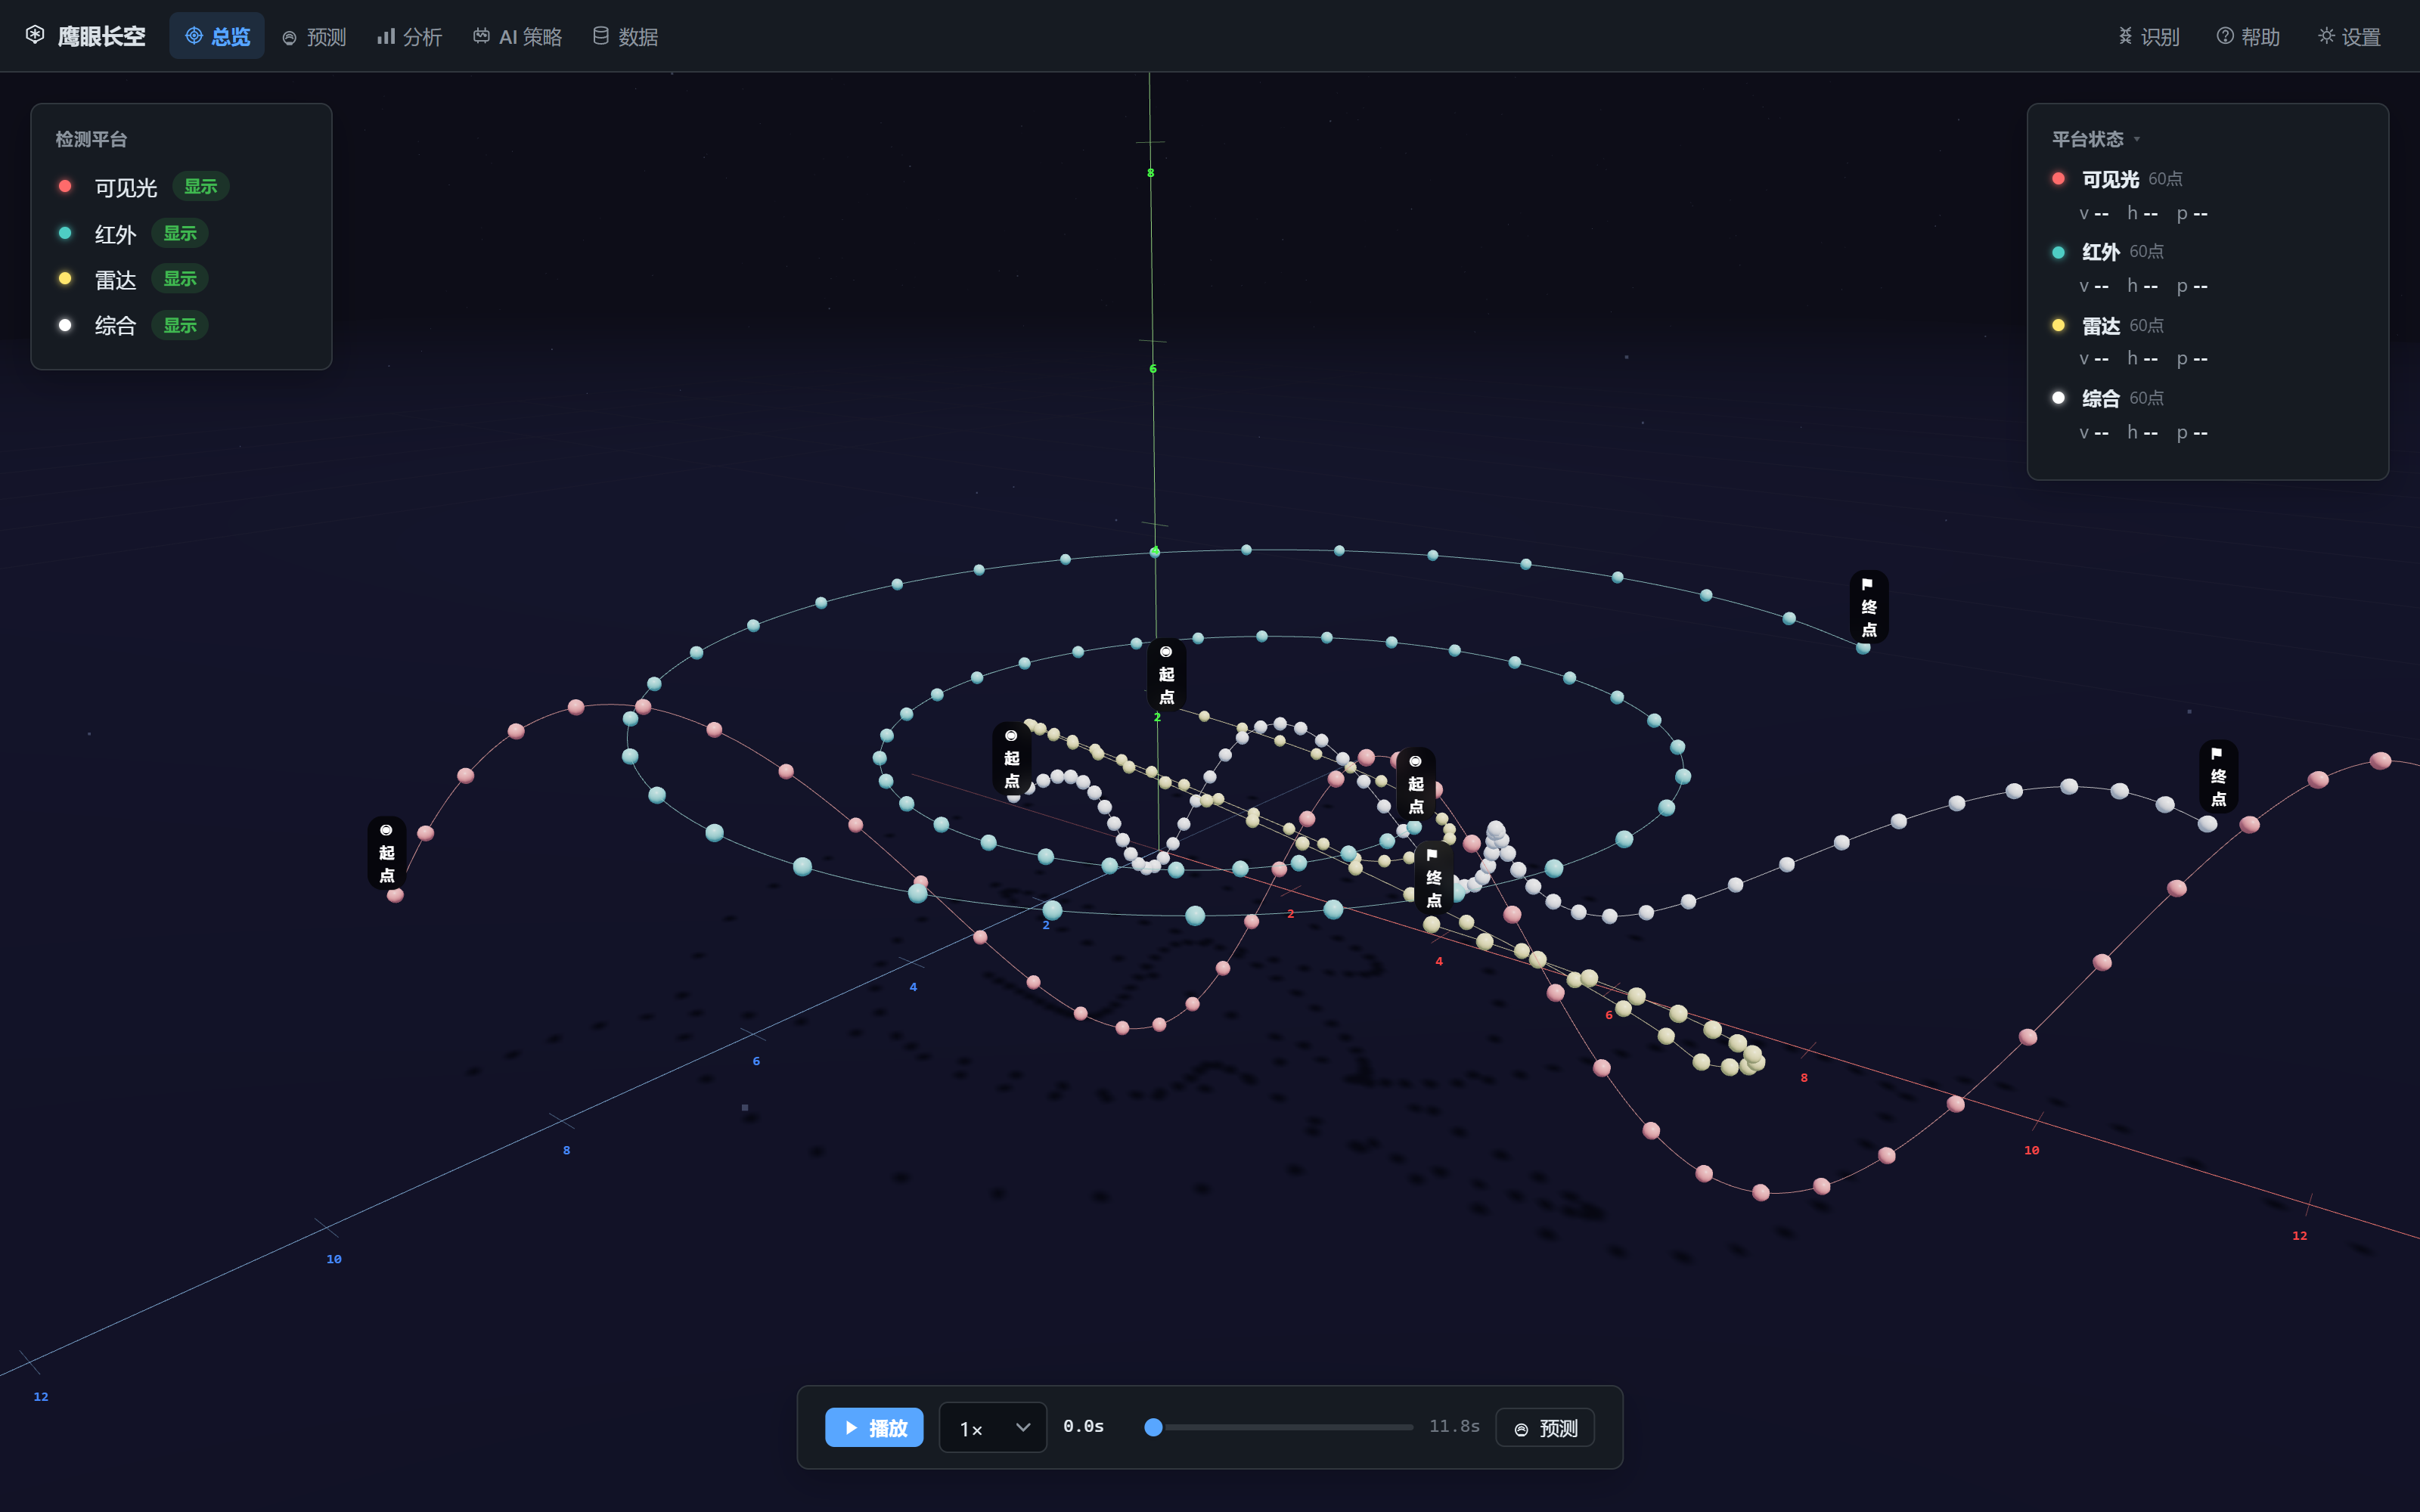
\includegraphics[width=\linewidth]{figures/ui/dashboard.png}};
\begin{scope}[x={(im.south east)},y={(im.north west)}]
  \hotspot{1}{0.115}{0.880}
  \hotspot{2}{0.945}{0.880}
  \hotspot{3}{0.500}{0.430}
  \hotspot{4}{0.345}{0.052}
  \hotspot{5}{0.640}{0.978}
\end{scope}
\end{tikzpicture}
\caption{总览页操作区域：\cn{1}~检测平台面板\quad \cn{2}~平台状态面板\quad \cn{3}~三维轨迹场景\quad \cn{4}~时间轴控制条\quad \cn{5}~顶部导航栏}
\label{fig:use_dashboard}
\end{figure}

\begin{enumerate}
  \item \term{检测平台面板（左上，\cn{1}）}：每一项左侧圆点为该平台颜色，右侧按钮切换“显示/隐藏”；隐藏只影响绘制，不删除数据。
  \item \term{平台状态面板（右上，\cn{2}）}：显示各平台点数与当前时刻的速度 $v$、高度 $h$、位置 $p$，随播放实时刷新；点击标题可折叠。
  \item \term{三维轨迹场景（\cn{3}）}：彩色曲线为各平台轨迹，白色为加权融合的综合轨迹；每条轨迹标注起点与终点，中央坐标轴标注 $X$（红）、$Y$（绿）、$Z$（蓝）。
  \item \term{时间轴控制条（\cn{4}）}：播放/暂停、倍速（0.5×--4×）、当前时刻、进度滑块与总时长；右侧“预测”按钮直达预测页。
  \item \term{顶部导航栏（\cn{5}）}：左侧五个主功能入口（总览、预测、分析、AI 策略、数据），右侧“识别 / 帮助 / 设置”；当前页面入口高亮。
\end{enumerate}

\subsubsection{三维视图操作}

\begin{table}[H]
\centering
\caption{三维视图与常用操作}
\label{tab:use_ops}
\small
\begin{tabularx}{\linewidth}{@{}>{\heiti}p{4.0cm}>{\raggedright\arraybackslash}X@{}}
\toprule
操作 & 效果 \\
\midrule
按住左键拖动 & 绕视点旋转，换角度观察轨迹 \\
滚动滚轮 & 拉近 / 拉远 \\
按住右键拖动 & 平移视点 \\
W / S / A / D & 相机前后左右移动 \\
Q / E & 相机下降 / 上升 \\
鼠标悬停轨迹点 & 球体放大并弹出该点坐标与时刻 \\
空格键 & 播放 / 暂停动画 \\
\bottomrule
\end{tabularx}
\end{table}

\begin{notebox}[两个实用技巧]
轨迹重叠时，先在左侧面板隐藏部分平台逐个观察；相机移动速度可在 \file{config.json} 的 \code{camera_speed} 中调整（默认 0.1）。所有操作结果以右下角浮层提示反馈：绿色成功、红色失败、黄色警告。
\end{notebox}

\subsection{轨迹重建与分析的操作}

\subsubsection{预测页}

预测页在历史轨迹之后叠加预测段（图~\ref{fig:use_predict}）。

\begin{figure}[H]
\centering
\begin{tikzpicture}
\node[inner sep=0, anchor=south west] (im) at (0,0)
  {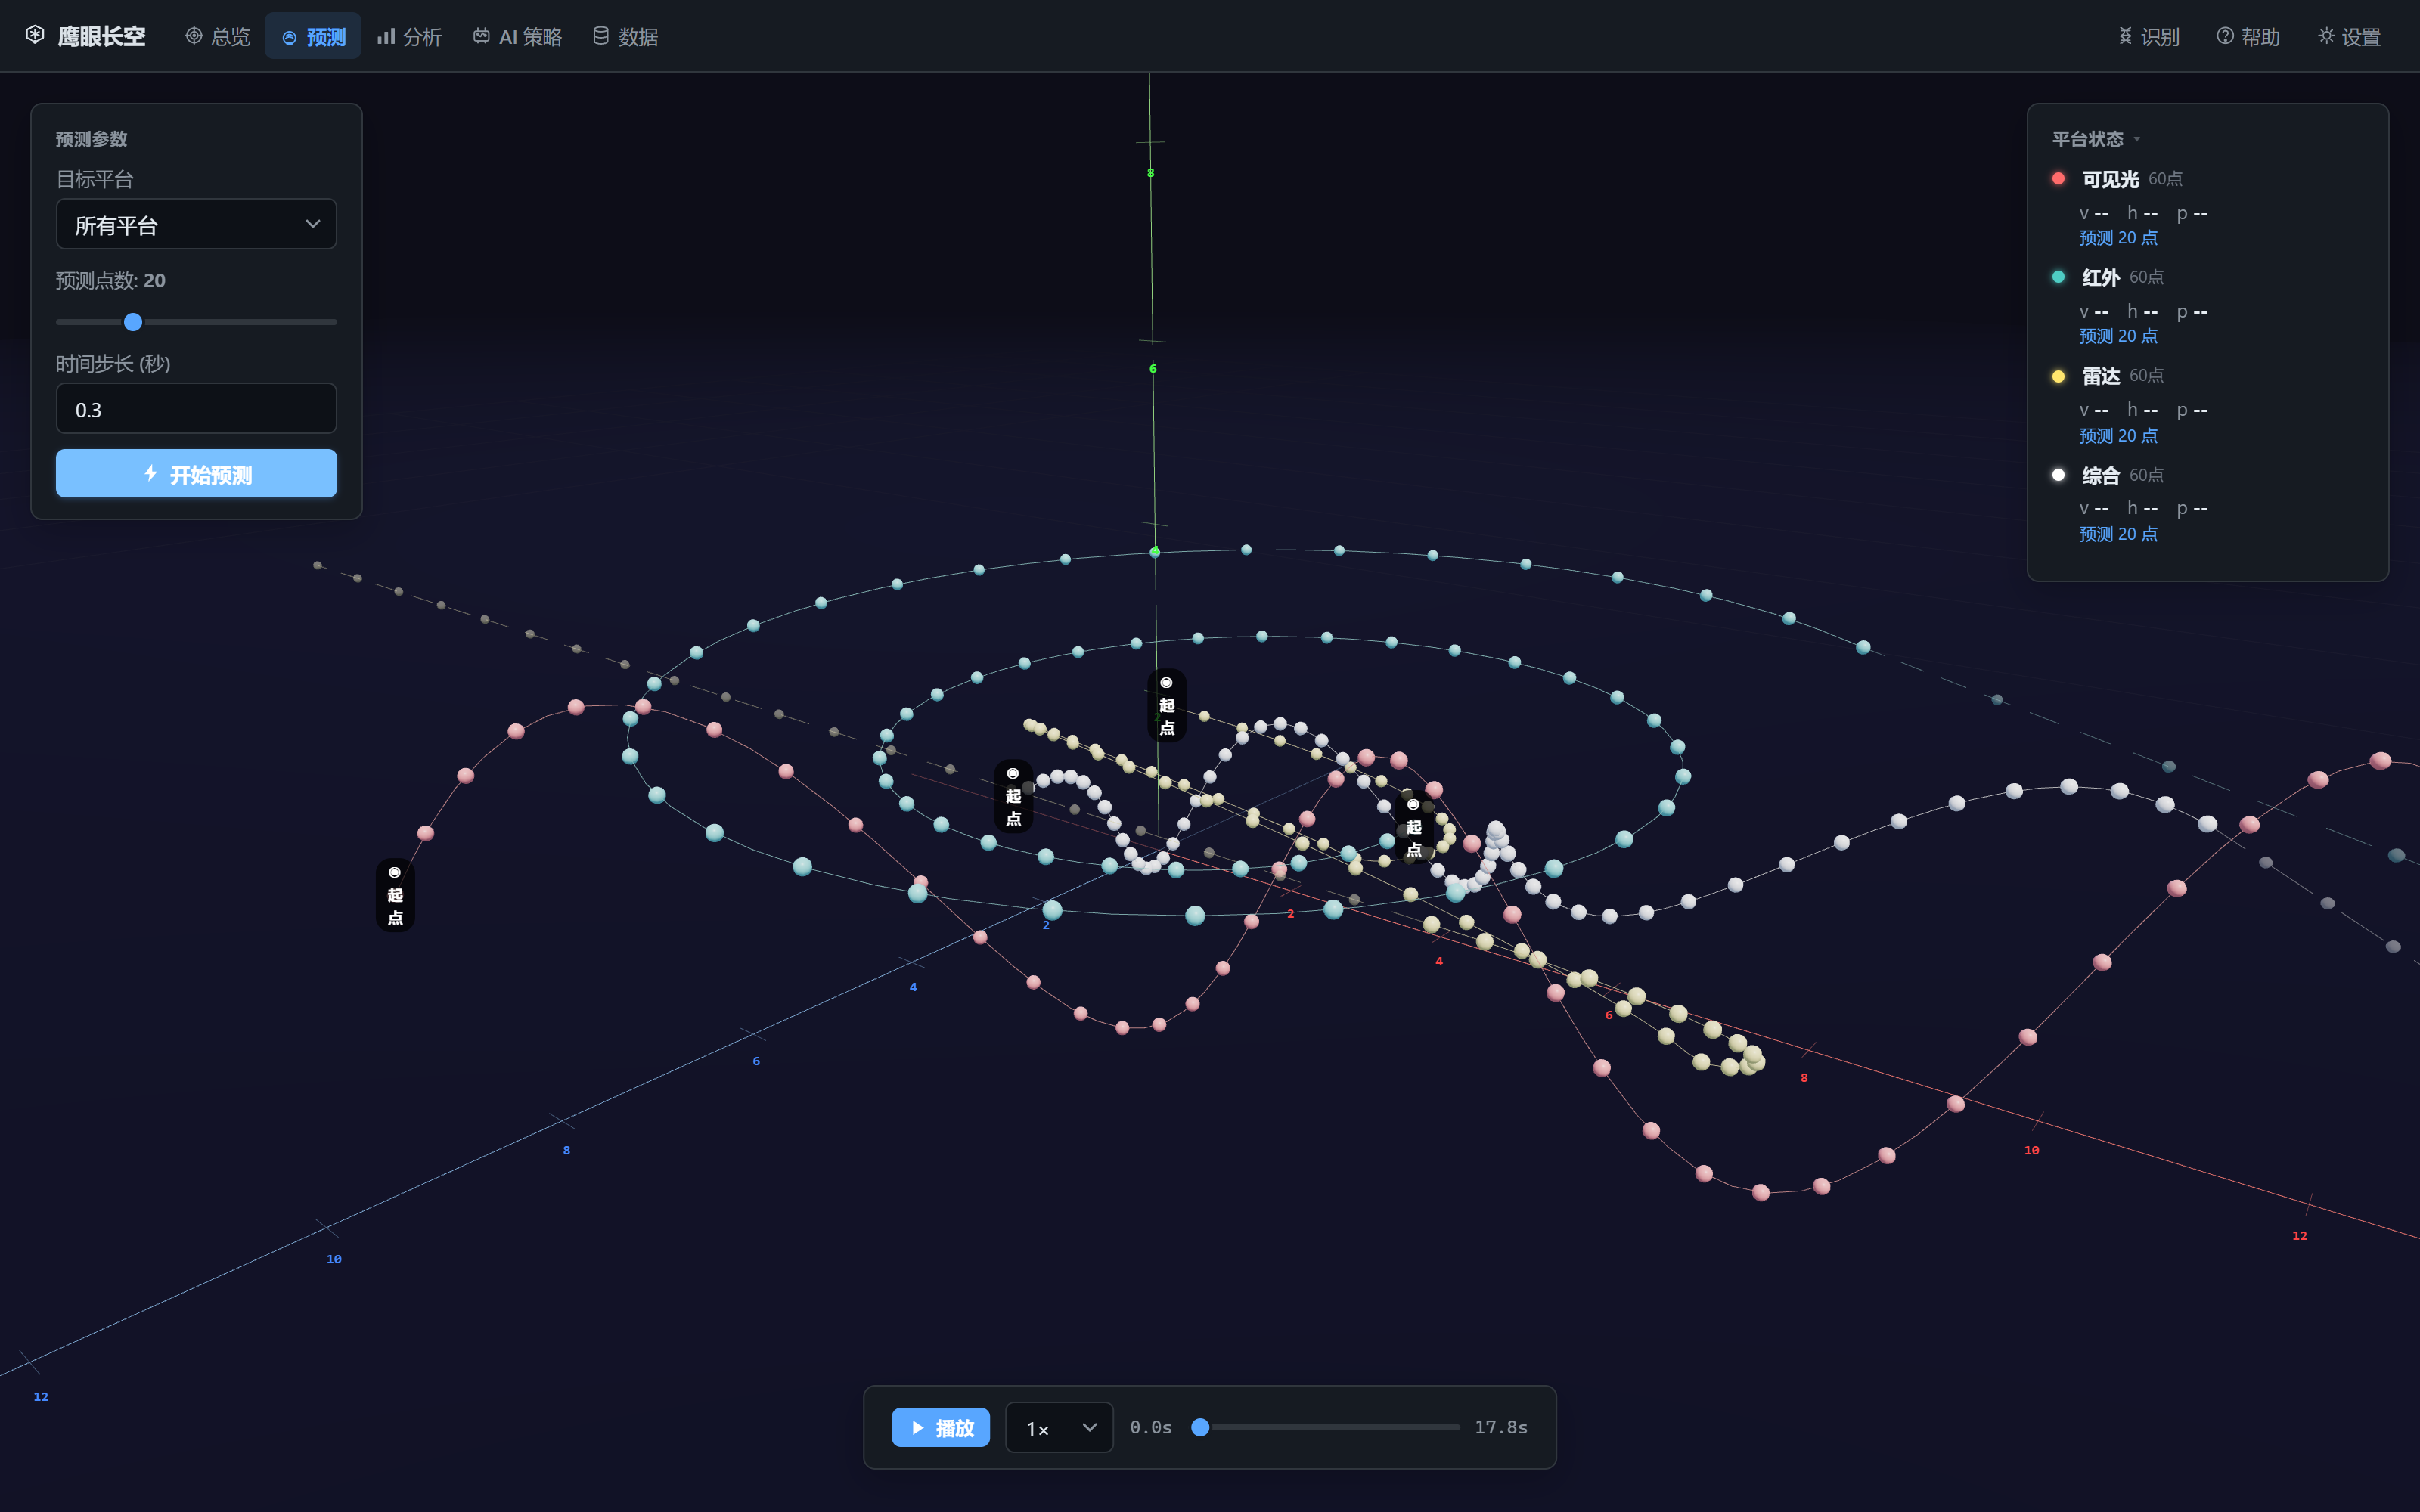
\includegraphics[width=\linewidth]{figures/ui/predict.png}};
\begin{scope}[x={(im.south east)},y={(im.north west)}]
  \hotspot{1}{0.133}{0.848}
  \hotspot{2}{0.133}{0.735}
  \hotspot{3}{0.960}{0.880}
  \hotspot{4}{0.170}{0.600}
  \hotspot{5}{0.335}{0.055}
\end{scope}
\end{tikzpicture}
\caption{预测页操作区域：\cn{1}~目标平台\quad \cn{2}~预测点数与步长\quad \cn{3}~平台状态（含预测点数）\quad \cn{4}~预测段（虚线）\quad \cn{5}~回放控制条}
\label{fig:use_predict}
\end{figure}

操作步骤：

\begin{enumerate}
  \item 在“目标平台”中选择单个平台或“所有平台”（\cn{1}）；
  \item 拖动“预测点数”滑块（10--50，默认 20），填写“时间步长”（默认 0.3 s）（\cn{2}）；
  \item 点击“开始预测”，场景中出现虚线预测段（\cn{4}），右上状态面板出现“预测 20 点”标注（\cn{3}）；
  \item 点击“播放”（\cn{5}），观察目标从历史段进入预测段的过渡是否平滑。
\end{enumerate}

\begin{notebox}[预测精度说明]
当前预测以线性外推兜底，即按最后两点的速度直线延伸，对转弯、加速等机动的描述能力有限；深度学习混合模型仍在完善中。预测结果适合判断大致走向，不宜作为精确拦截依据。
\end{notebox}

\subsubsection{分析页}

分析页把轨迹拆成四条曲线，并给出最适宜处置的三个时刻（图~\ref{fig:use_analysis}）。

\begin{figure}[H]
\centering
\begin{tikzpicture}
\node[inner sep=0, anchor=south west] (im) at (0,0)
  {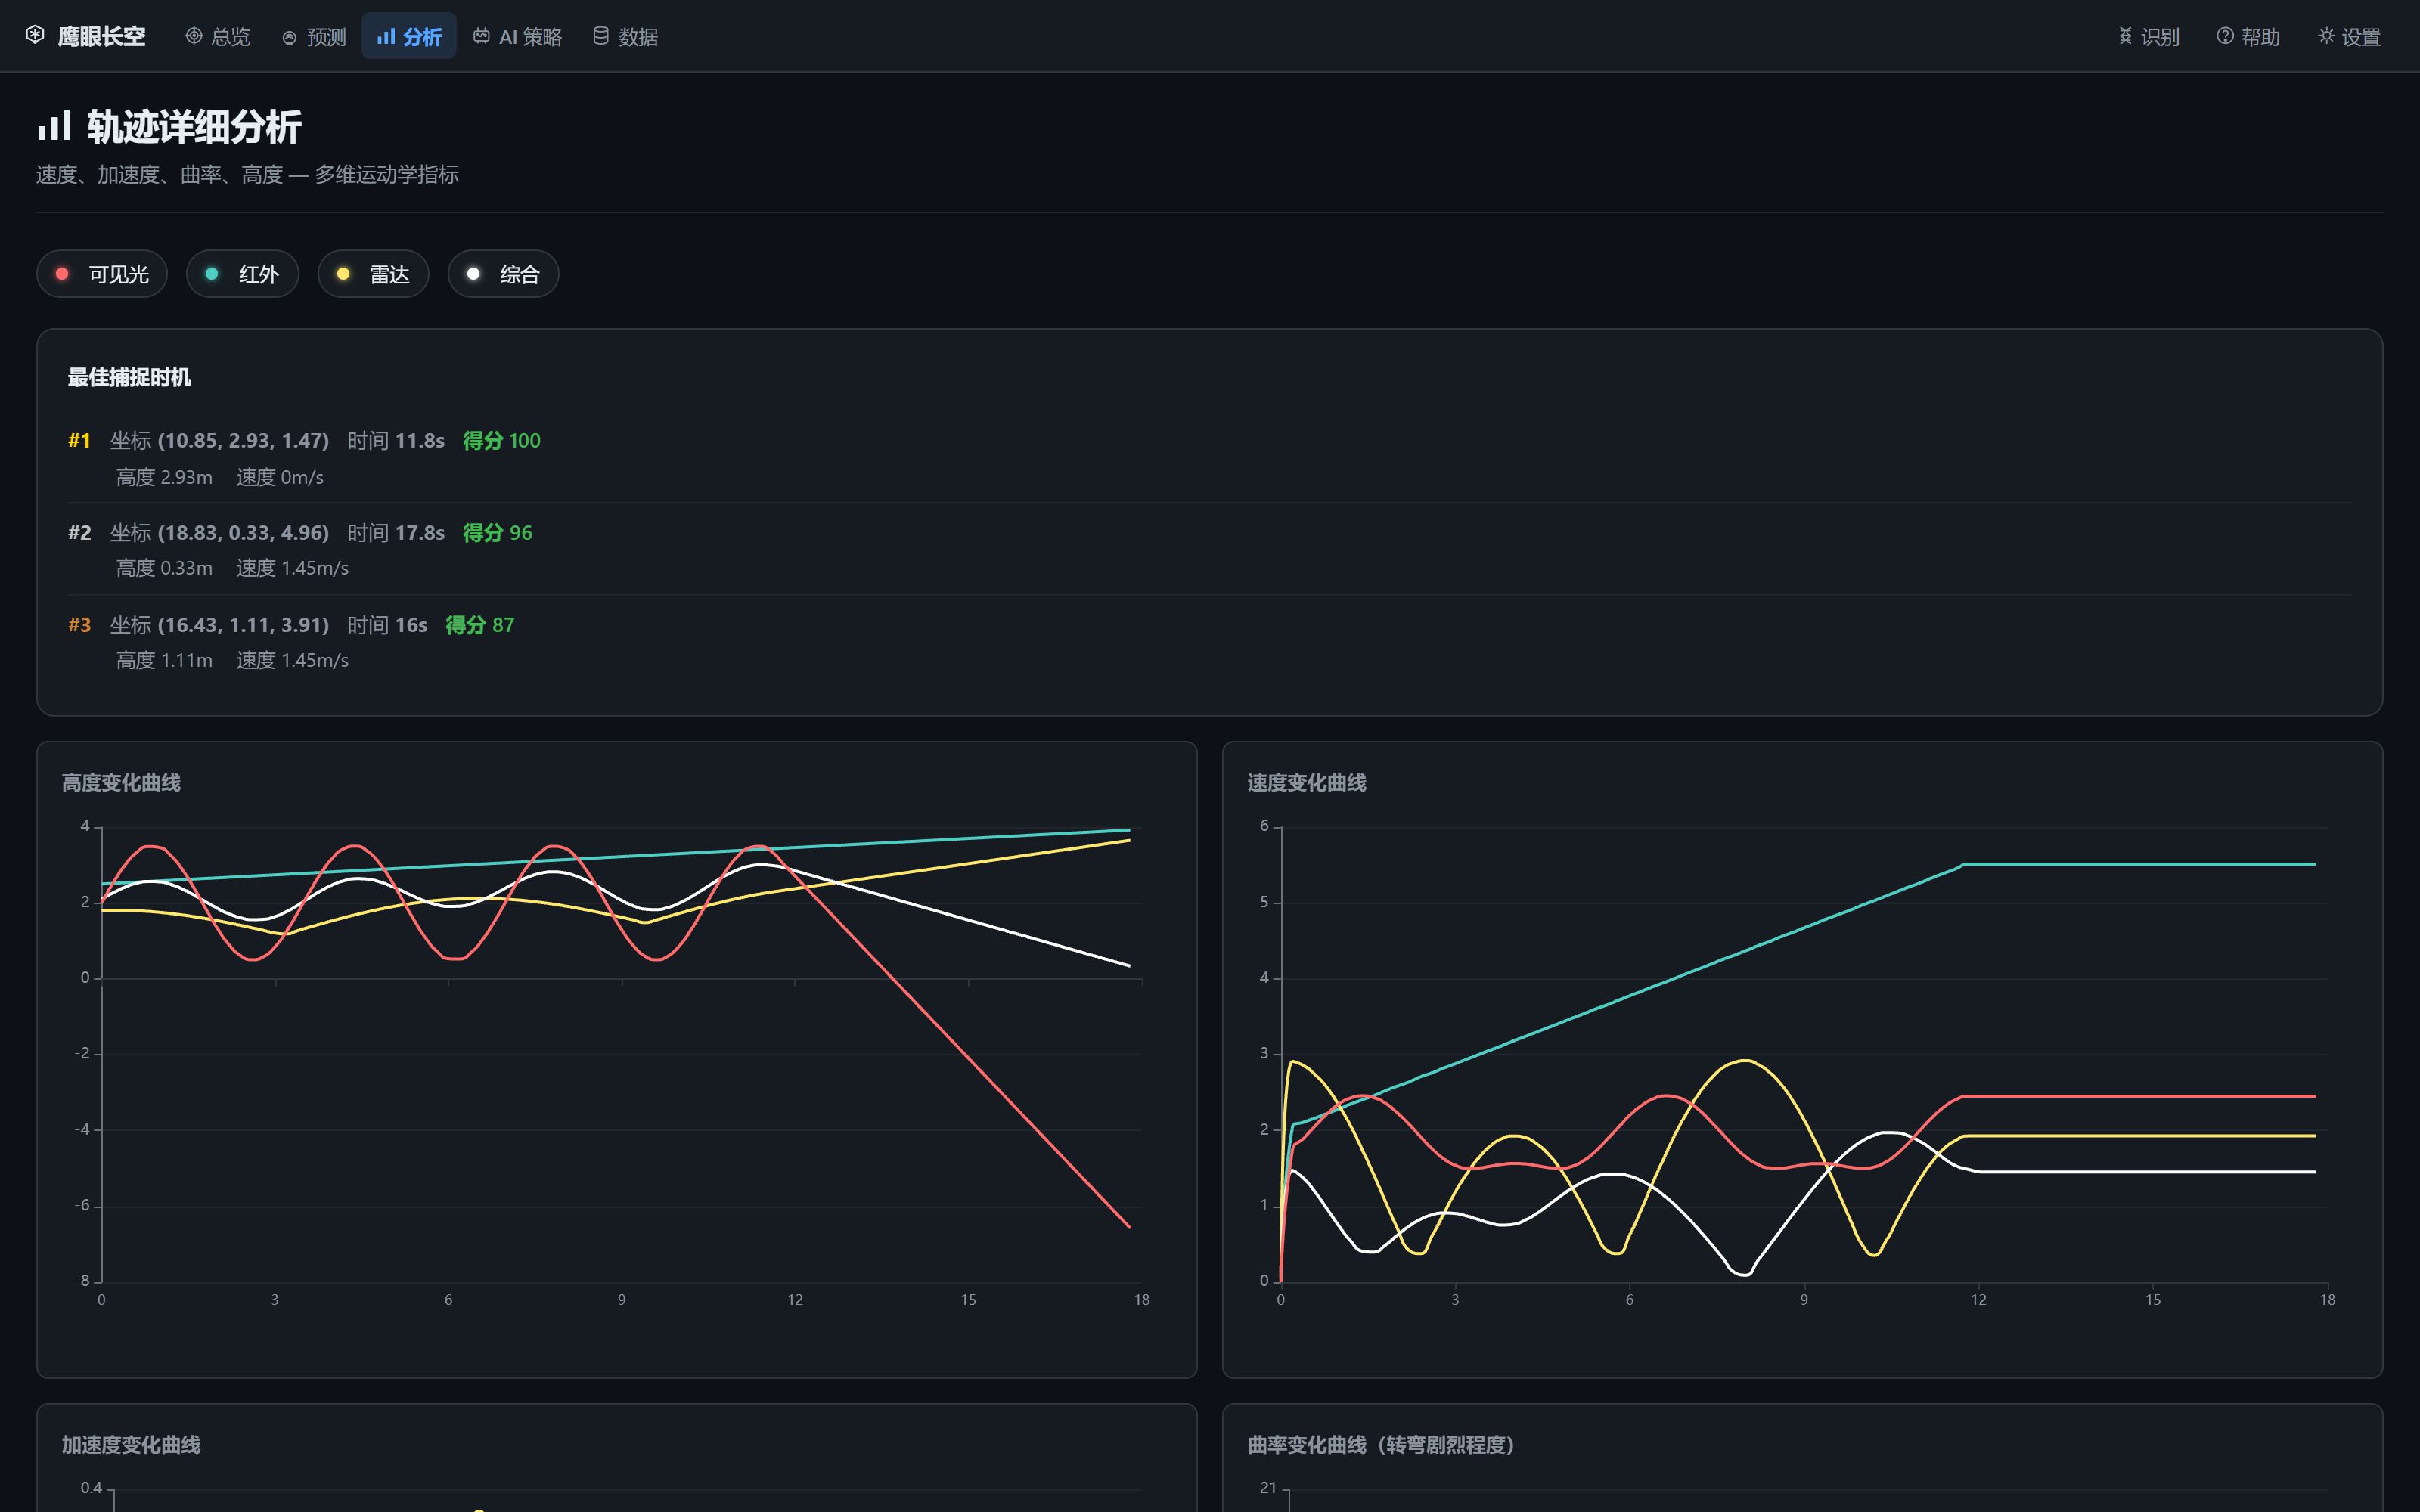
\includegraphics[width=\linewidth]{figures/ui/analysis.png}};
\begin{scope}[x={(im.south east)},y={(im.north west)}]
  \hotspot{1}{0.300}{0.805}
  \hotspot{2}{0.600}{0.720}
  \hotspot{3}{0.440}{0.600}
  \hotspot{4}{0.945}{0.600}
\end{scope}
\end{tikzpicture}
\caption{分析页操作区域：\cn{1}~平台筛选\quad \cn{2}~最佳捕捉时机\quad \cn{3}~高度/速度曲线\quad \cn{4}~加速度/曲率曲线}
\label{fig:use_analysis}
\end{figure}

\begin{enumerate}
  \item \term{平台筛选（\cn{1}）}：点击彩色标签只看某一平台，便于横向对比；默认全部显示。
  \item \term{最佳捕捉时机（\cn{2}）}：列出得分前三的时刻、坐标、得分（最高 100）、高度与速度；“越低、越慢、越平稳、航线越直”得分越高。
  \item \term{高度/速度曲线（\cn{3}）}：曲线末端为预测段，若出现陡降或突跳，说明预测偏离物理常识，应谨慎采信。
  \item \term{加速度/曲率曲线（\cn{4}）}：两者同时出现峰值，通常表示目标正在急转机动。
\end{enumerate}

\begin{notebox}[使用前提]
捕捉时机依赖预测数据：需先在预测页执行一次预测，否则该卡片为空。切换页面或重启后预测文件会被清空，需重新预测。
\end{notebox}

\subsubsection{AI 策略页}

AI 策略页把勾选平台的轨迹提交大模型，生成反制建议（图~\ref{fig:use_ai}）。

\begin{figure}[H]
\centering
\begin{tikzpicture}
\node[inner sep=0, anchor=south west] (im) at (0,0)
  {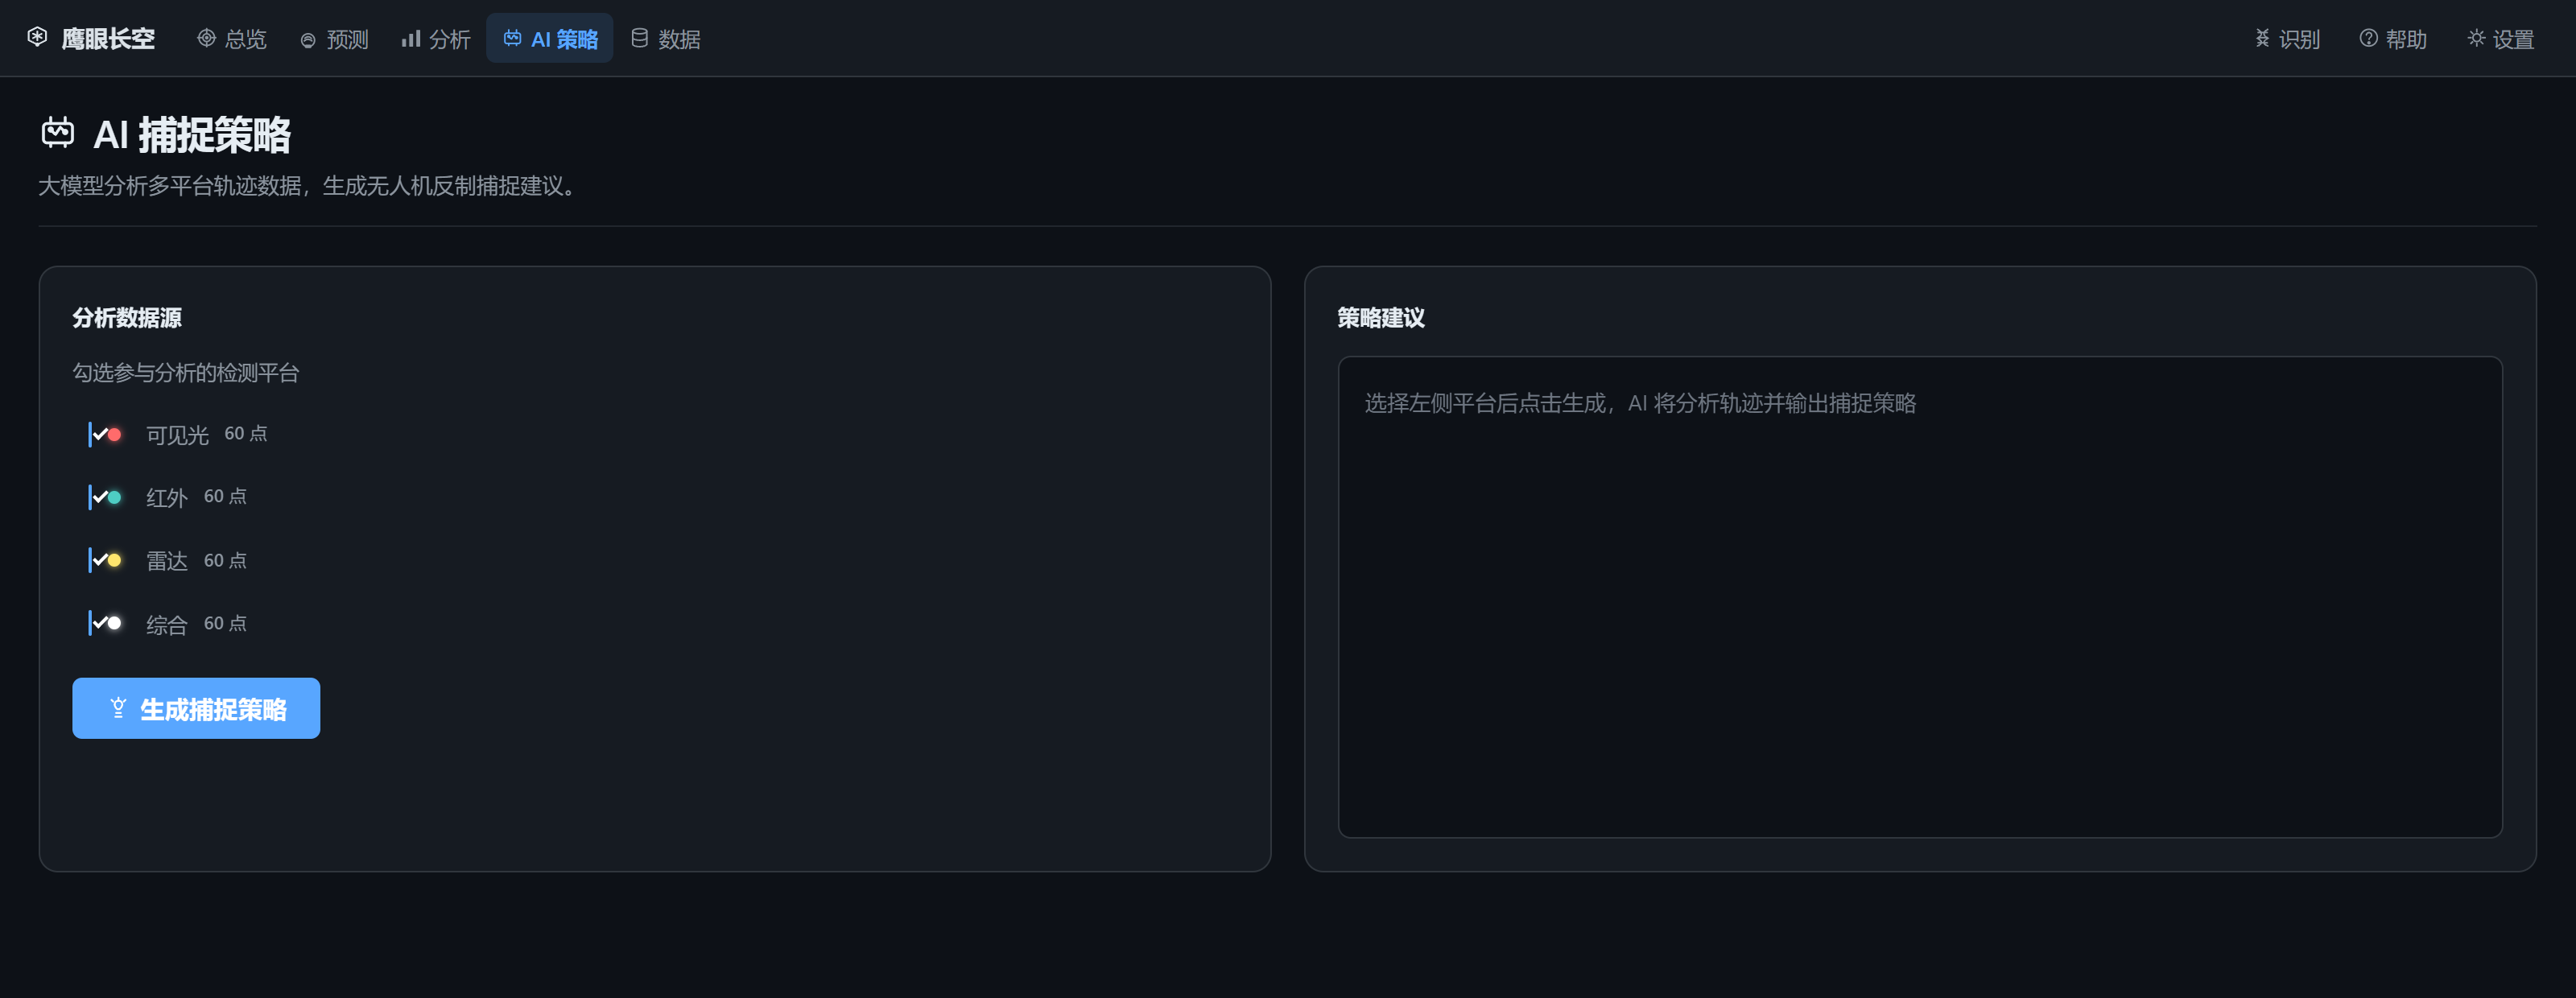
\includegraphics[width=\linewidth]{figures/ui/ai.png}};
\begin{scope}[x={(im.south east)},y={(im.north west)}]
  \hotspot{1}{0.300}{0.520}
  \hotspot{2}{0.155}{0.320}
  \hotspot{3}{0.800}{0.300}
\end{scope}
\end{tikzpicture}
\caption{AI 策略页操作区域：\cn{1}~平台勾选\quad \cn{2}~生成按钮\quad \cn{3}~策略输出区}
\label{fig:use_ai}
\end{figure}

\begin{enumerate}
  \item 勾选参与分析的平台（\cn{1}），建议一次勾选 2--3 个，避免提示词过长；
  \item 点击“生成捕捉策略”（\cn{2}），等待期间按钮显示加载状态；
  \item 返回的建议显示在右侧（\cn{3}），可点击“保存为报告”存入 \file{reports/}，文件名带时间戳。
\end{enumerate}

若提示“AI 服务异常”，请先检查 \file{config.json} 中 \code{ai} 段的地址、密钥与模型名，并确认网络可访问该接口。

\subsubsection{数据管理页}

数据页负责数据上传与备份恢复（图~\ref{fig:use_data}）。

\begin{figure}[H]
\centering
\begin{tikzpicture}
\node[inner sep=0, anchor=south west] (im) at (0,0)
  {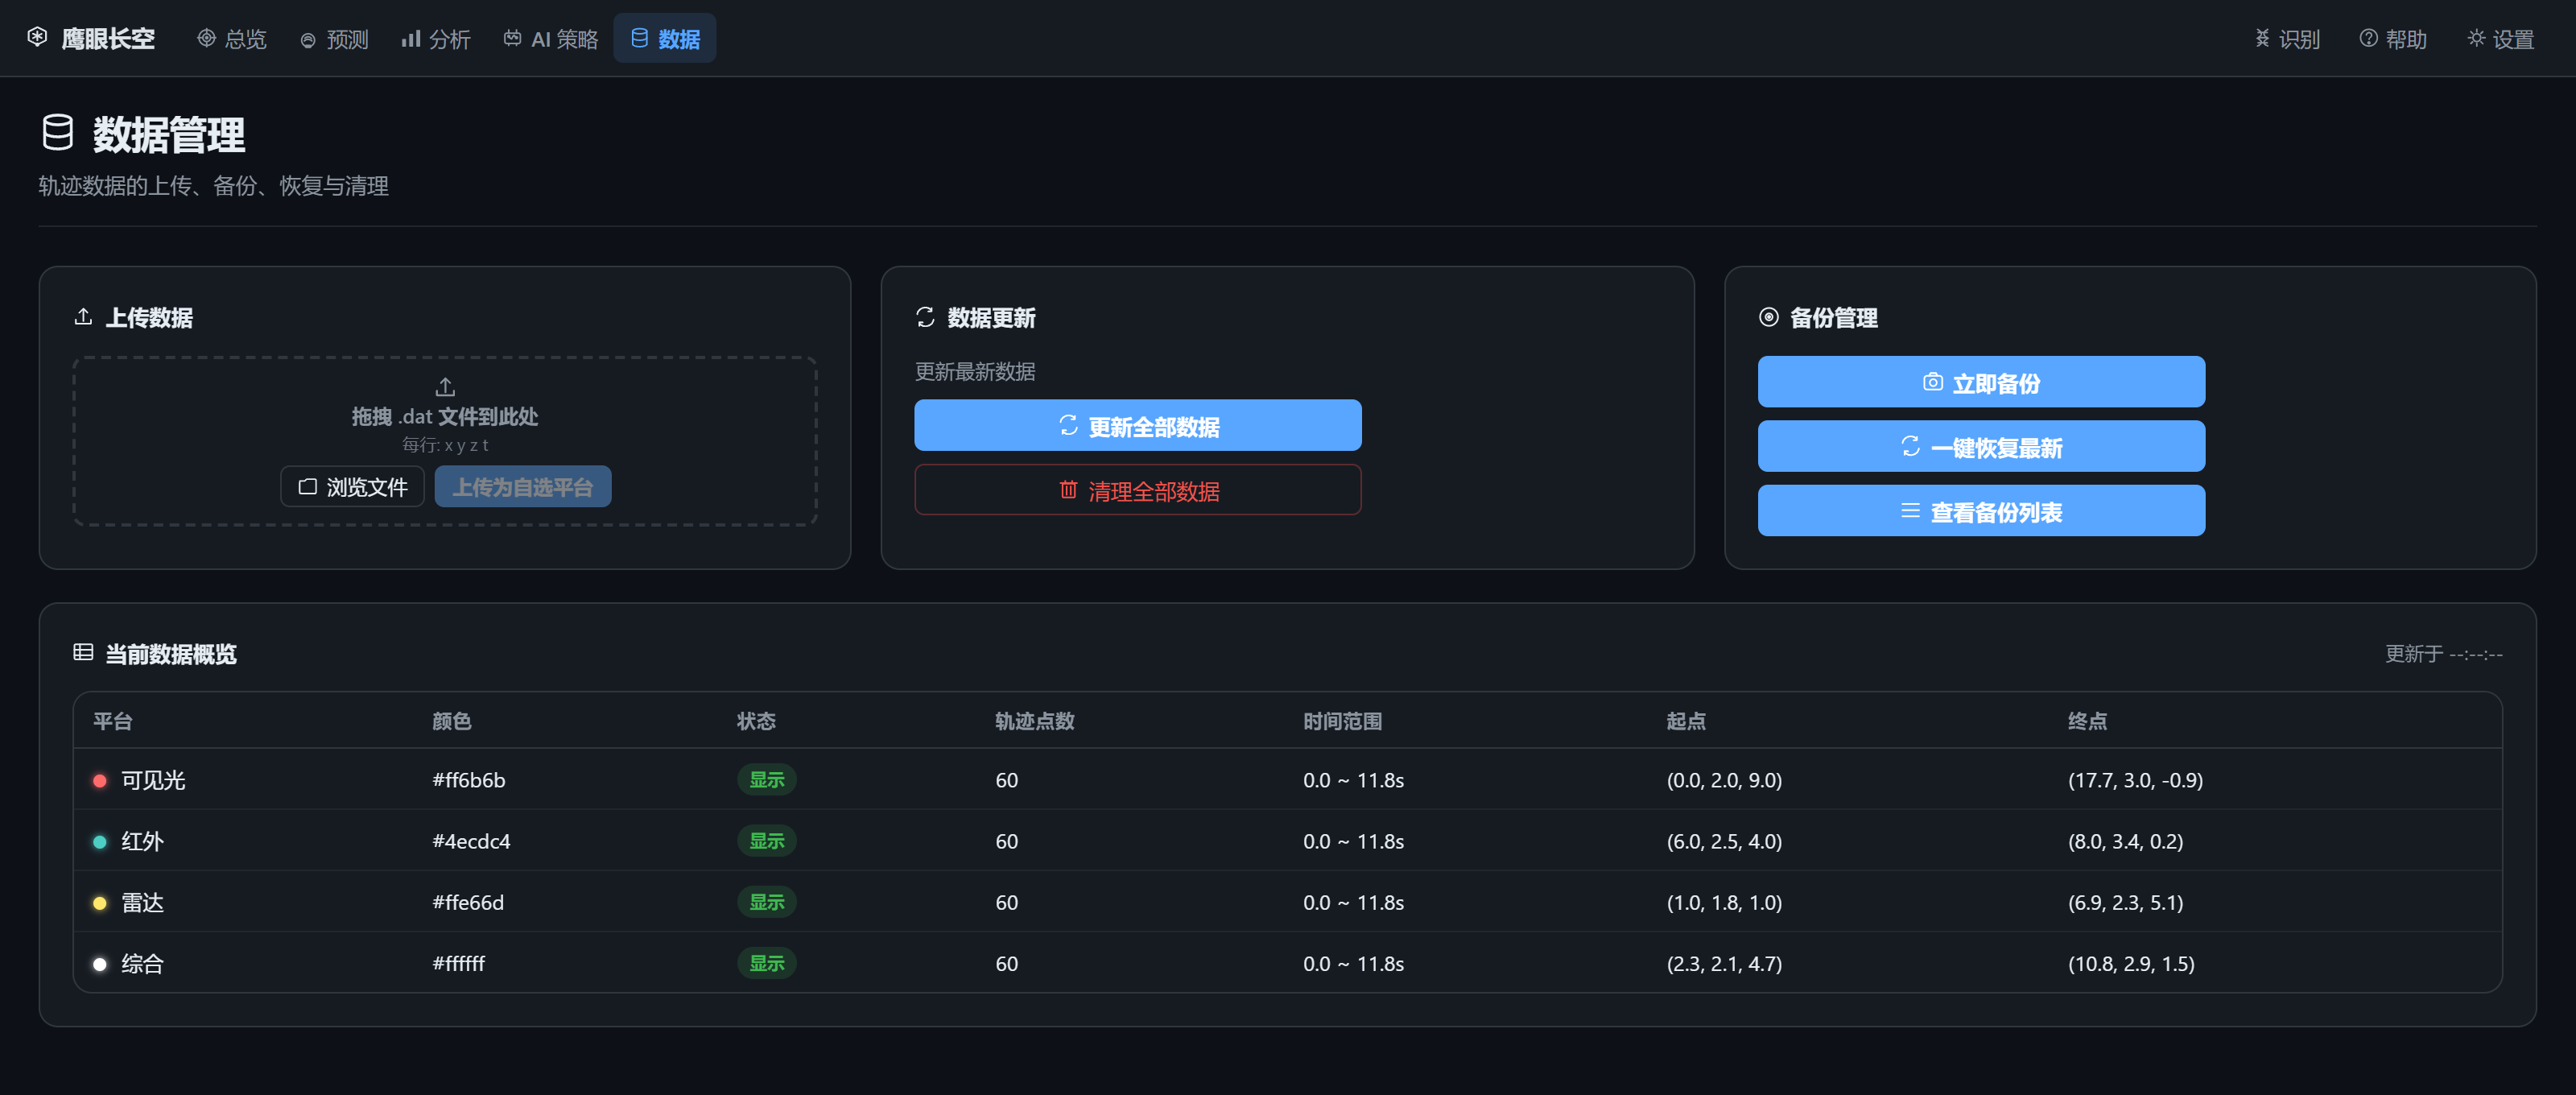
\includegraphics[width=\linewidth]{figures/ui/data.png}};
\begin{scope}[x={(im.south east)},y={(im.north west)}]
  \hotspot{1}{0.315}{0.815}
  \hotspot{2}{0.635}{0.815}
  \hotspot{3}{0.955}{0.815}
  \hotspot{4}{0.145}{0.400}
\end{scope}
\end{tikzpicture}
\caption{数据管理页操作区域：\cn{1}~上传自选数据\quad \cn{2}~数据更新与清理\quad \cn{3}~备份管理\quad \cn{4}~数据概览}
\label{fig:use_data}
\end{figure}

\begin{enumerate}
  \item \term{上传自选数据（\cn{1}）}：把每行 \code{x y z t} 的 \file{.dat} 文件拖入虚线框，或点击“浏览文件”；成功后出现新的“自选”平台。
  \item \term{数据更新与清理（\cn{2}）}：“更新全部数据”重新读取事实轨迹并重算综合轨迹；“清理全部数据”会先自动备份再清空，用于演示复位。
  \item \term{备份管理（\cn{3}）}：“立即备份”生成快照；“一键恢复最新”回到最近快照；“查看备份列表”可做部分恢复或删除。
  \item \term{数据概览（\cn{4}）}：逐平台显示颜色、状态、点数、时间范围、起点与终点，用于核对数据。
\end{enumerate}

\begin{notebox}[两种恢复方式]
\term{部分恢复}只覆盖快照中存在的文件，适合找回单个平台；\term{完整恢复}先清空现有数据再释放快照，适合回到某个历史状态。恢复后软件自动重算综合轨迹。
\end{notebox}

\subsubsection{设置页}

设置页调整主题、平台权重与评分权重（图~\ref{fig:use_settings}）。

\begin{figure}[H]
\centering
\begin{tikzpicture}
\node[inner sep=0, anchor=south west] (im) at (0,0)
  {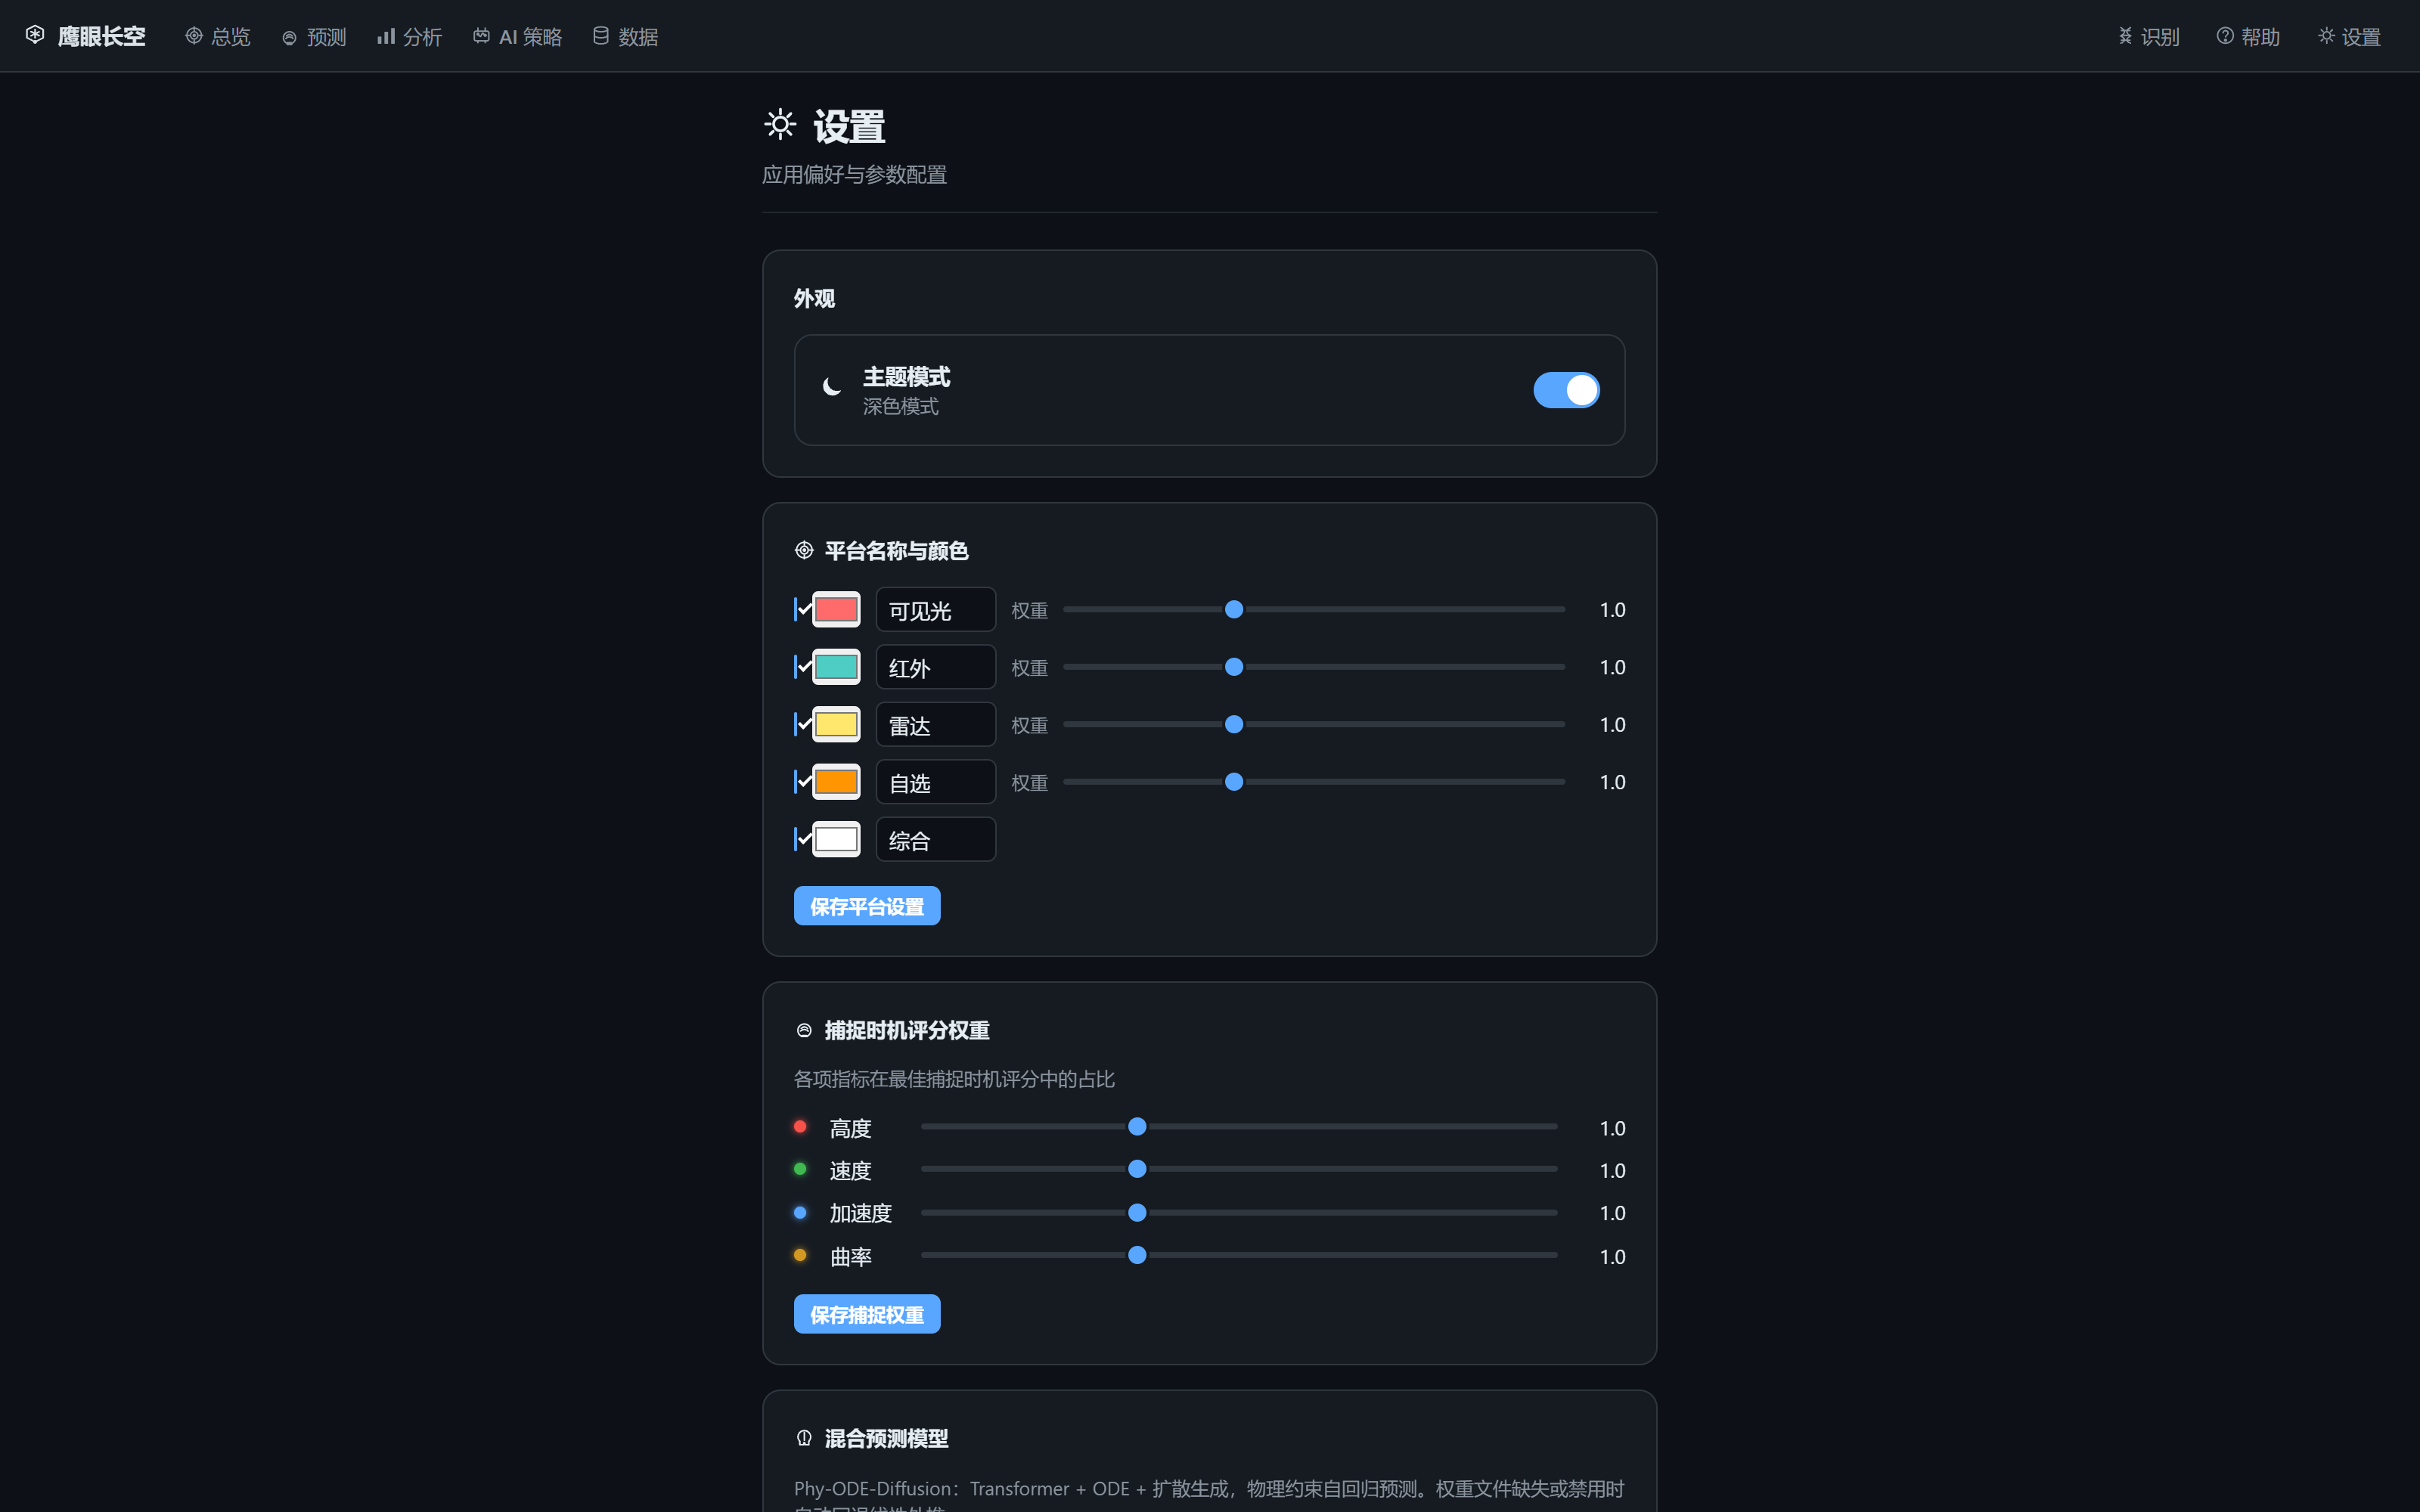
\includegraphics[width=\linewidth]{figures/ui/settings.png}};
\begin{scope}[x={(im.south east)},y={(im.north west)}]
  \hotspot{1}{0.600}{0.800}
  \hotspot{2}{0.600}{0.630}
  \hotspot{3}{0.600}{0.310}
\end{scope}
\end{tikzpicture}
\caption{设置页操作区域：\cn{1}~主题切换\quad \cn{2}~平台名称、颜色与权重\quad \cn{3}~捕捉评分权重}
\label{fig:use_settings}
\end{figure}

\begin{enumerate}
  \item \term{主题切换（\cn{1}）}：深色/浅色一键切换，立即生效并记住选择。
  \item \term{平台设置（\cn{2}）}：可改名称、颜色与融合权重；权重越大对综合轨迹影响越大，设为 0 即不参与融合。
  \item \term{捕捉权重（\cn{3}）}：调整高度、速度、加速度、曲率在评分中的比重，例如更看重低空就调大高度权重。
\end{enumerate}

设置页下方的“混合预测模型”区块用于调整最大速度、加速度、高度范围与推理步数等物理约束，保存后下一次预测生效。

\subsection{无人机检测的操作}

\subsubsection{检测工作台}

工作台自下而上分为视频源、检测控制、双目预览与实时信息四部分（图~\ref{fig:use_detect}）。

\begin{figure}[H]
\centering
\begin{tikzpicture}
\node[inner sep=0, anchor=south west] (im) at (0,0)
  {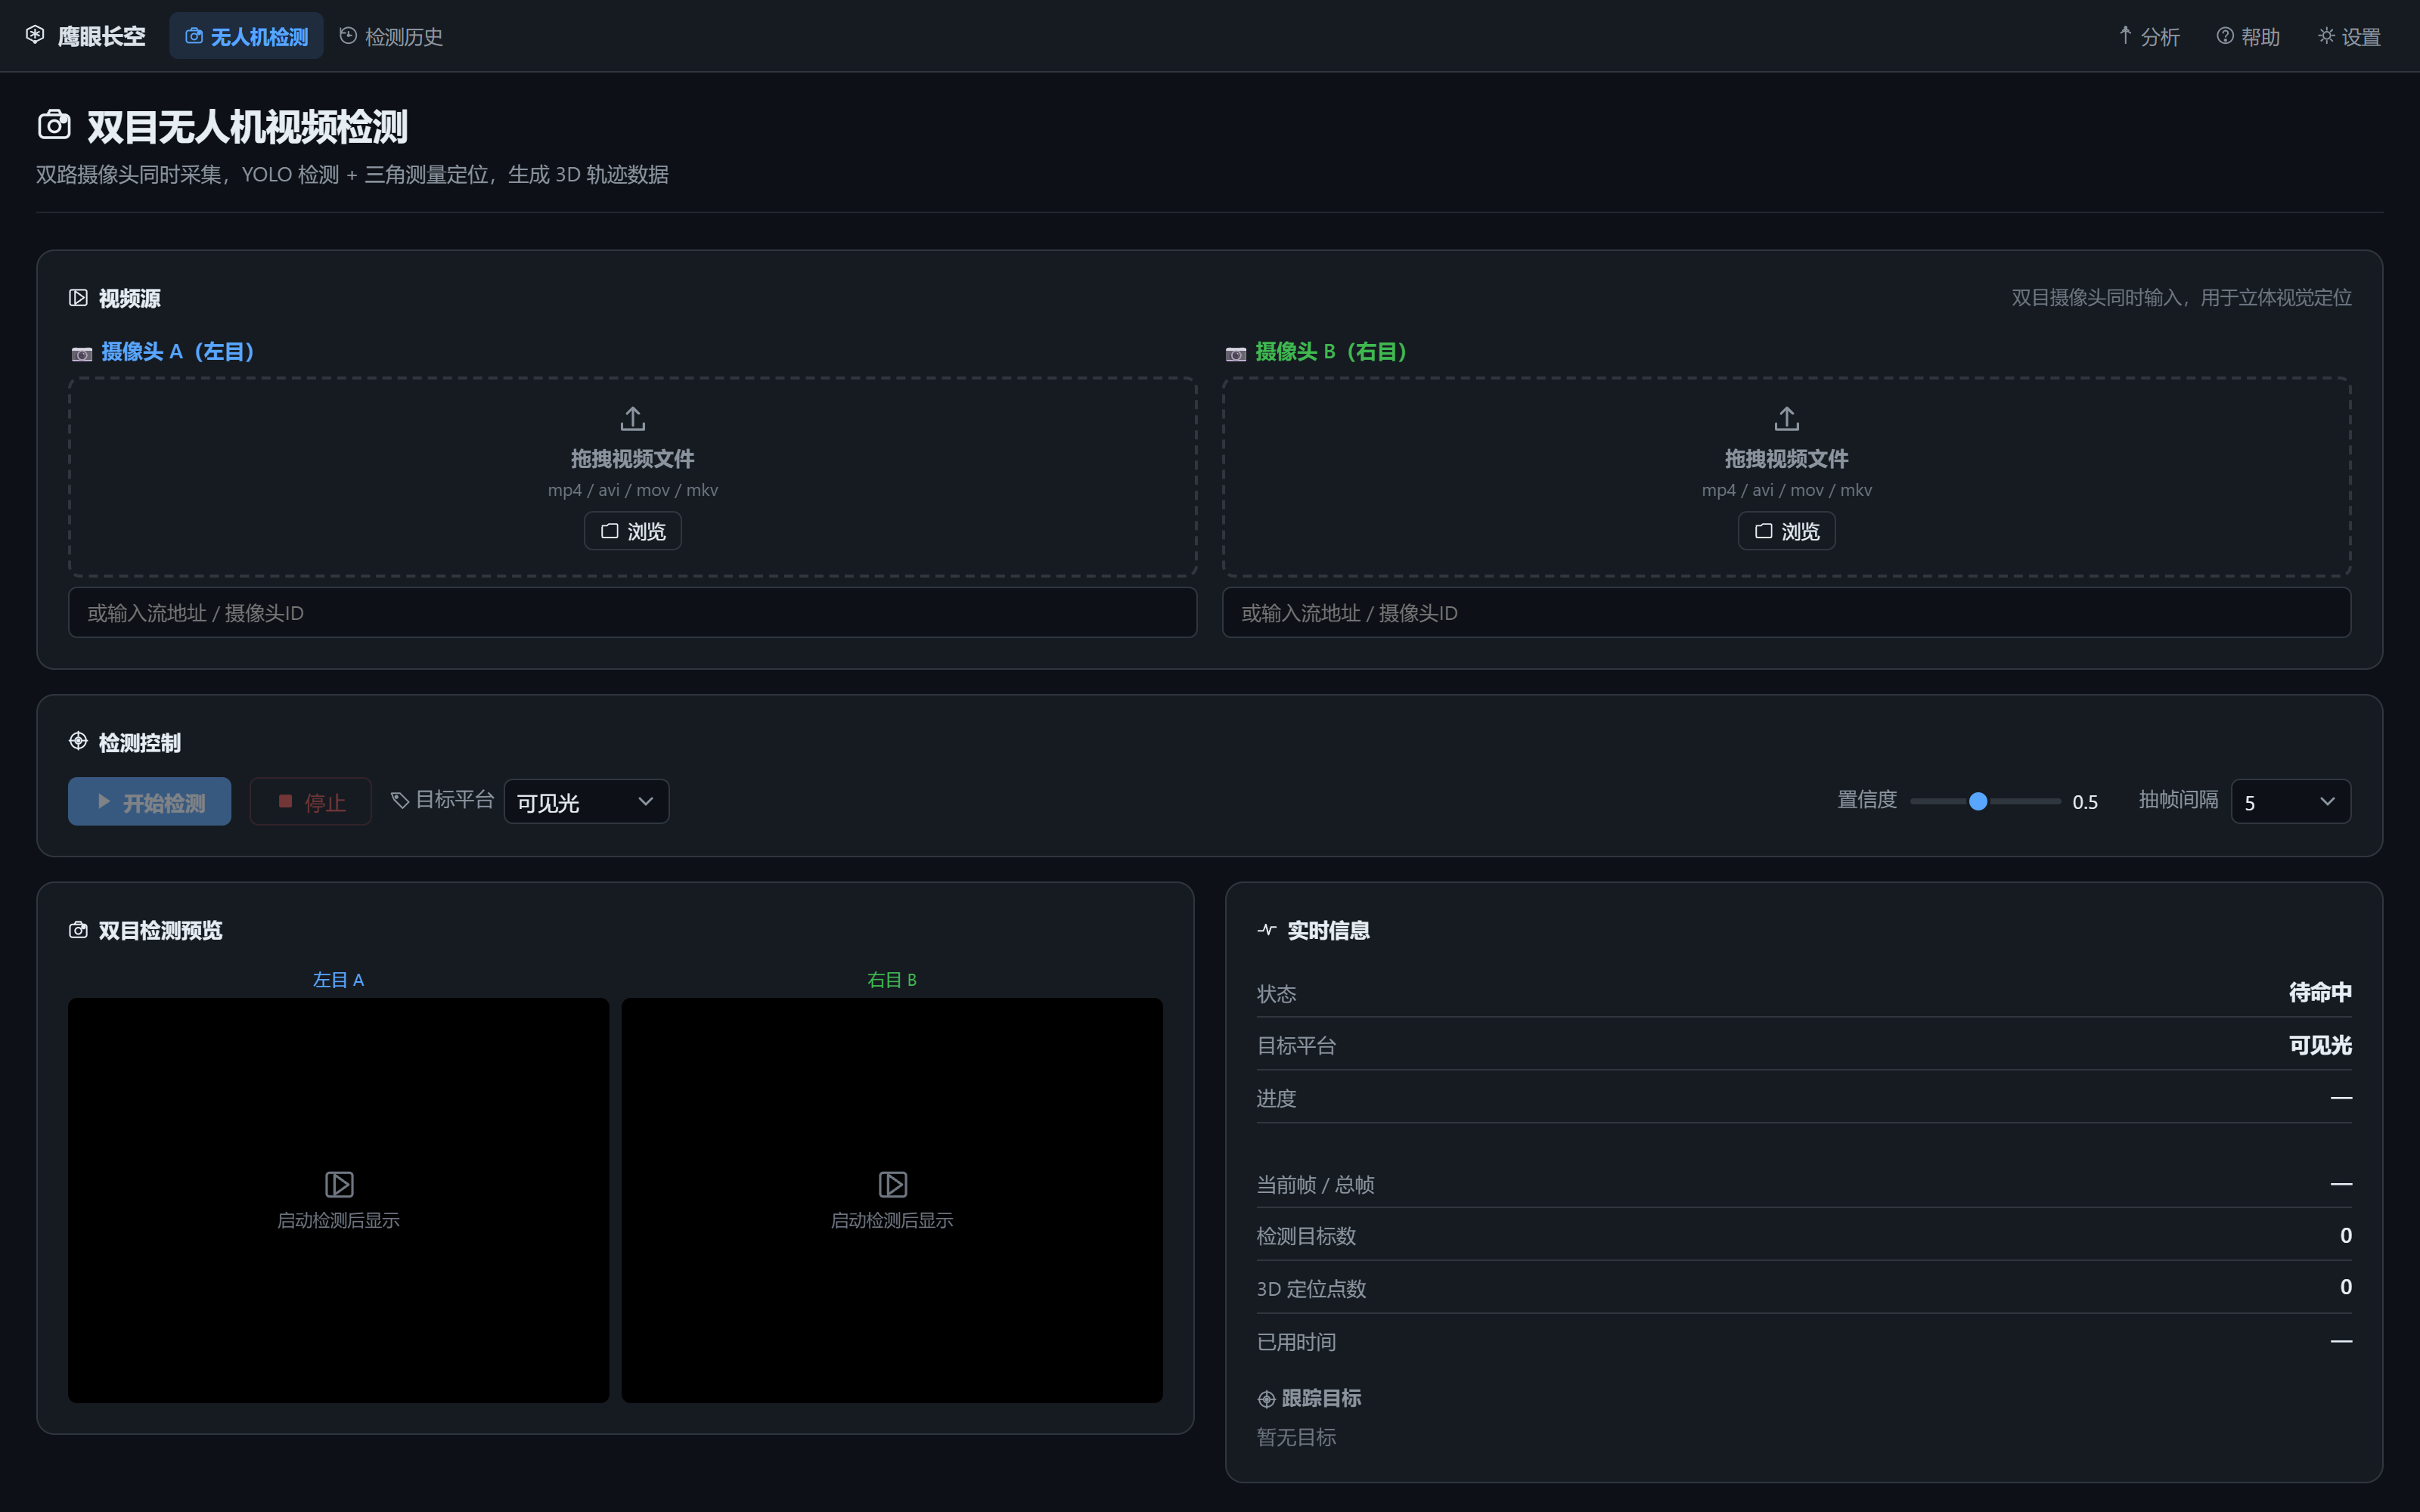
\includegraphics[width=\linewidth]{figures/ui/detect.png}};
\begin{scope}[x={(im.south east)},y={(im.north west)}]
  \hotspot{1}{0.300}{0.810}
  \hotspot{2}{0.350}{0.490}
  \hotspot{3}{0.440}{0.395}
  \hotspot{4}{0.945}{0.395}
\end{scope}
\end{tikzpicture}
\caption{检测工作台操作区域：\cn{1}~视频源上传\quad \cn{2}~检测控制条\quad \cn{3}~双目预览\quad \cn{4}~实时信息面板}
\label{fig:use_detect}
\end{figure}

\begin{enumerate}
  \item \term{视频源（\cn{1}）}：左右目各一个虚线框，可拖入视频文件（mp4/avi/mov/mkv），也可在下方填写 RTSP/HTTP 流地址或摄像头编号（如 \code{0}、\code{1}）。两路视频应来自同一时刻的双目相机，分辨率与帧率尽量一致。
  \item \term{检测控制（\cn{2}）}：开始/停止按钮、目标平台选择、置信度滑块与抽帧间隔；置信度越低越易检出但误检增多，抽帧间隔越大处理越快、轨迹越疏。
  \item \term{双目预览（\cn{3}）}：并排显示左右目画面，检测框上标注“类别 + 置信度”。
  \item \term{实时信息（\cn{4}）}：显示状态、进度、当前帧/总帧、目标数、三维点数、已用时与跟踪目标列表。
\end{enumerate}

操作步骤：拖入双路视频 → 选择目标平台 → 按需调整置信度与抽帧间隔 → 点击“开始检测” → 完成后点击“保存结果”（开启自动保存则无需此步）→ 回到总览页刷新即可看到新轨迹。

\begin{notebox}[检测没有结果怎么办]
先确认视频能正常播放；再检查设置页中的模型文件是否存在、目标类别是否与模型匹配；最后可把置信度调低到 0.1 重试。画面中明显有目标却完全没有框，多半是类别不匹配。
\end{notebox}

\subsubsection{检测设置}

\begin{figure}[H]
\centering
\begin{tikzpicture}
\node[inner sep=0, anchor=south west] (im) at (0,0)
  {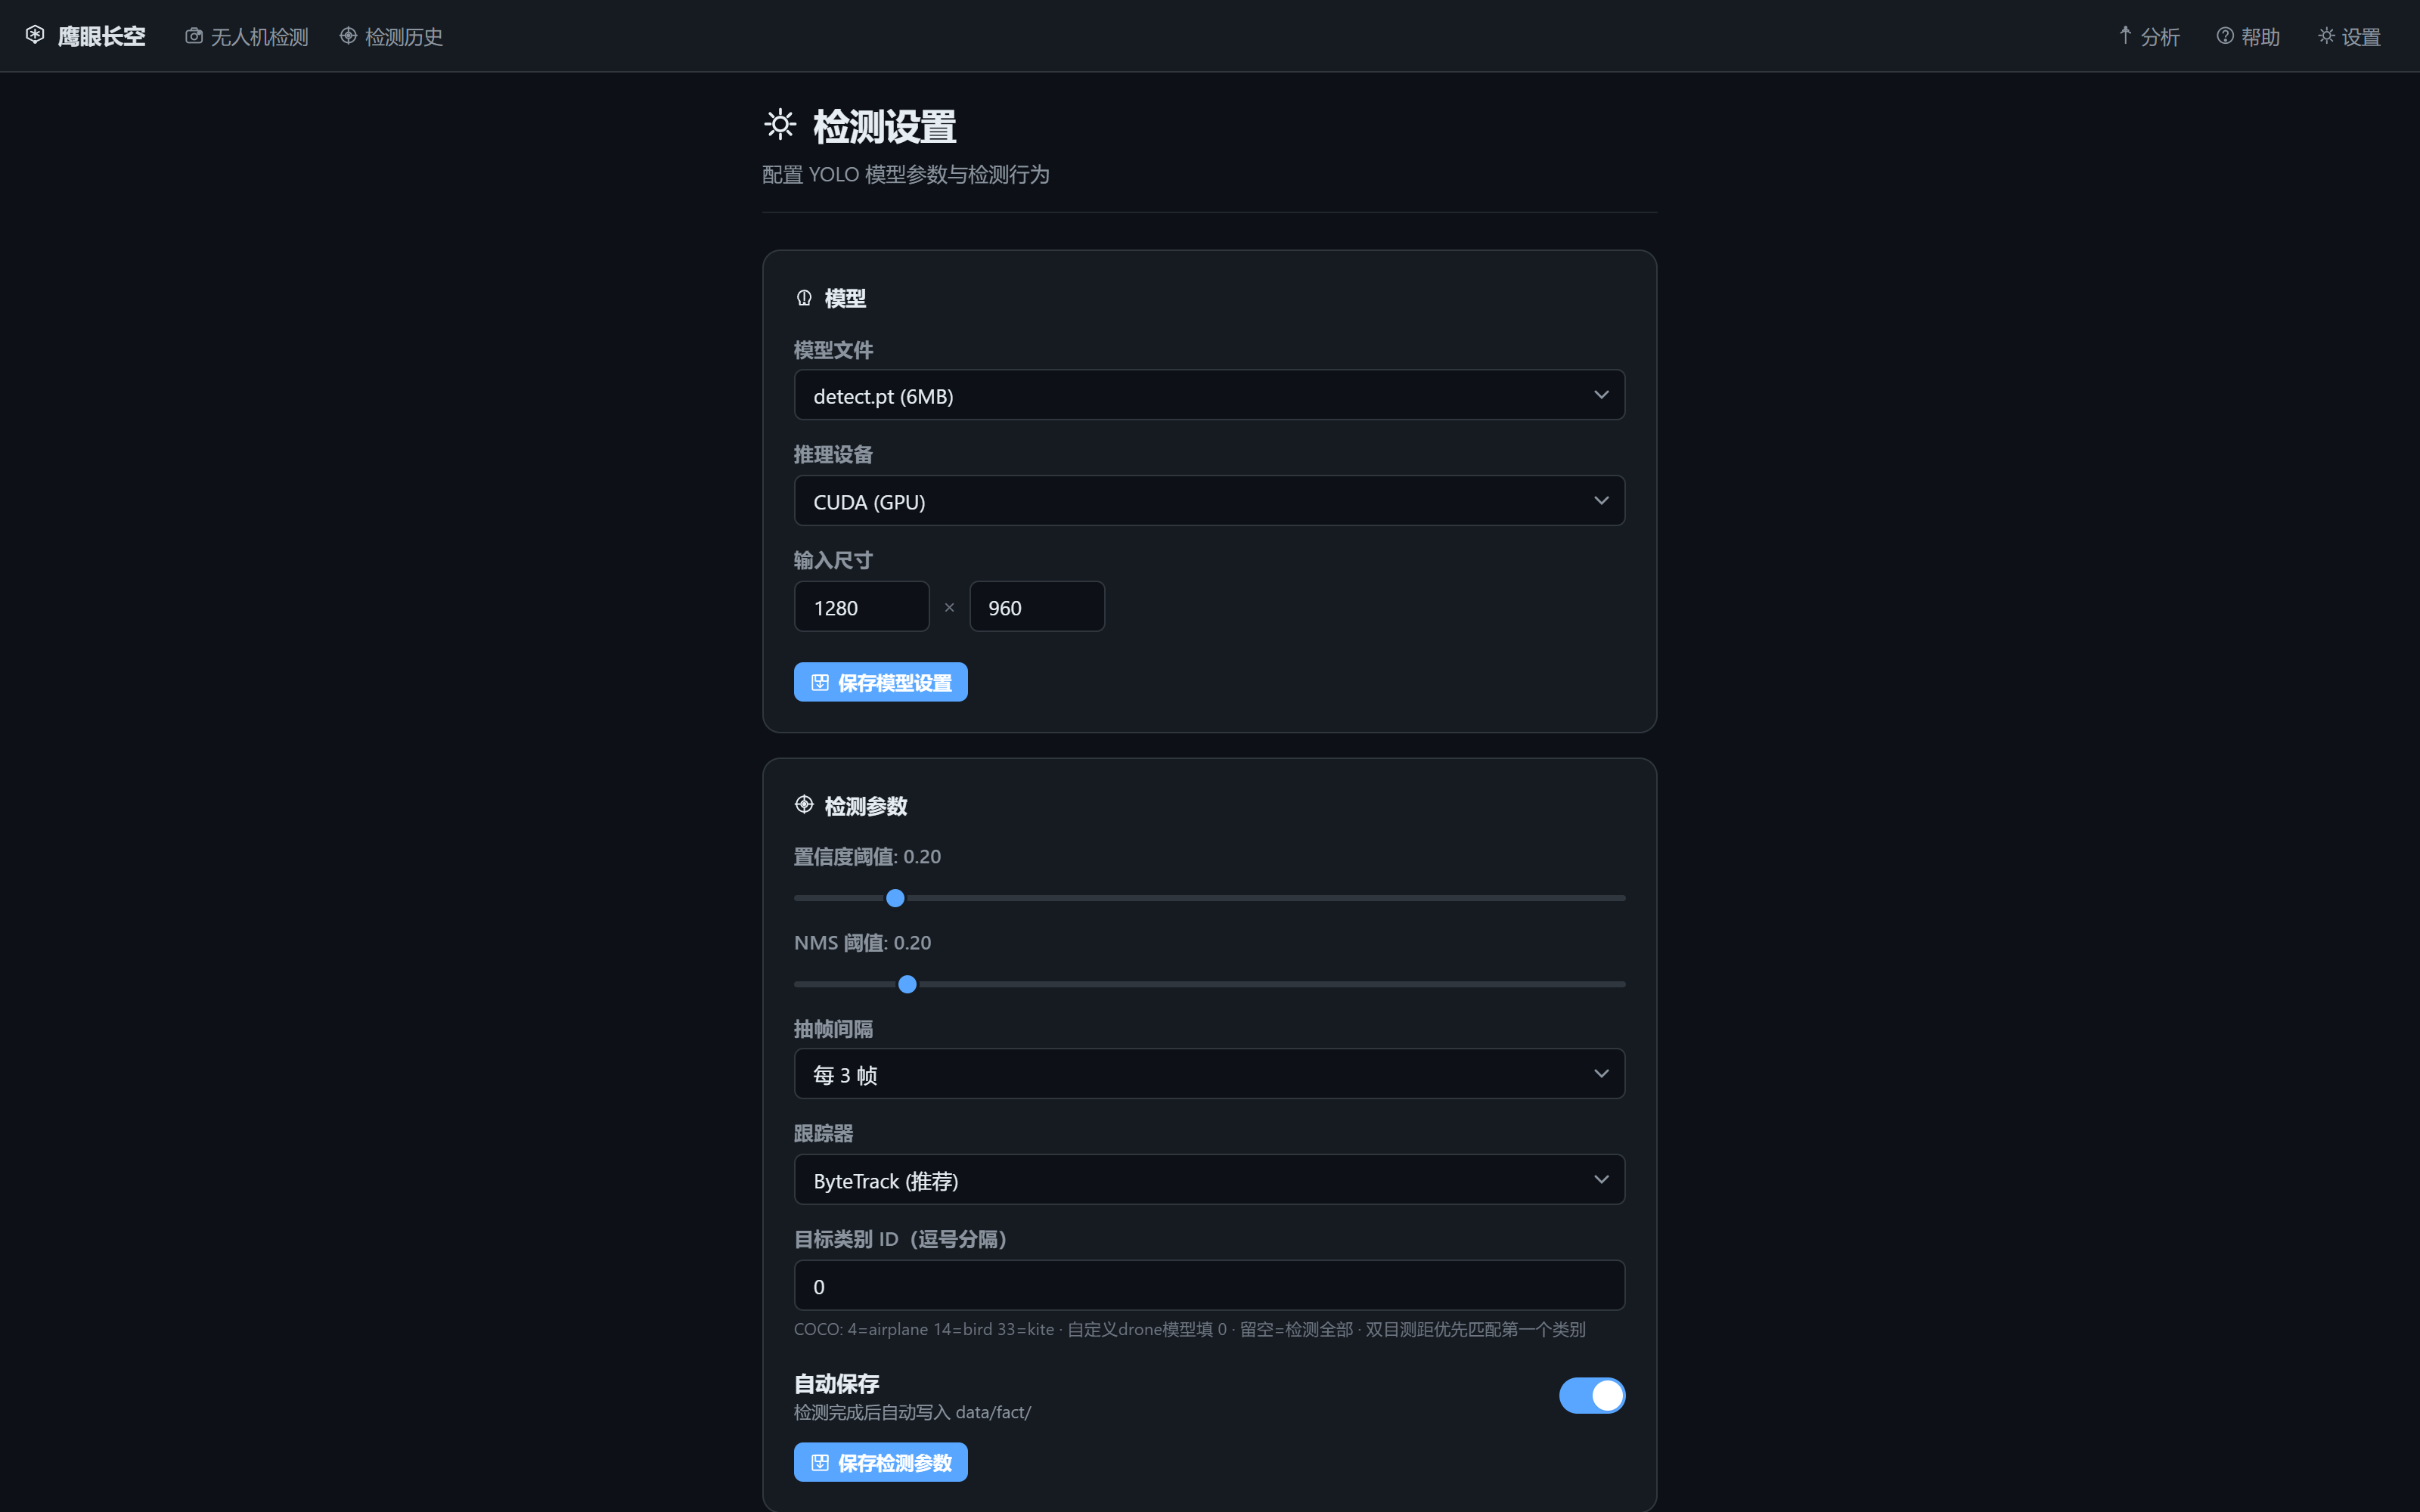
\includegraphics[width=\linewidth]{figures/ui/detect_settings.png}};
\begin{scope}[x={(im.south east)},y={(im.north west)}]
  \hotspot{1}{0.600}{0.800}
  \hotspot{2}{0.600}{0.470}
  \hotspot{3}{0.580}{0.080}
\end{scope}
\end{tikzpicture}
\caption{检测设置页操作区域：\cn{1}~模型与设备\quad \cn{2}~检测参数\quad \cn{3}~自动保存}
\label{fig:use_detect_settings}
\end{figure}

\begin{enumerate}
  \item \term{模型与设备（\cn{1}）}：选择 \file{models/yolo/} 中的权重；有 NVIDIA 显卡时选 CUDA 明显更快；输入尺寸一般保持 1280×960。
  \item \term{检测参数（\cn{2}）}：置信度、NMS、抽帧间隔、跟踪器与目标类别 ID。类别须与模型一致：自训练无人机模型通常为 0，COCO 预训练模型中飞机为 4、鸟为 14。
  \item \term{自动保存（\cn{3}）}：开启后检测完成即自动写入轨迹文件。
\end{enumerate}

修改后点击对应的“保存”按钮，参数立即写入 \file{config.json}，下一次检测生效。

\subsubsection{检测历史}

\begin{figure}[H]
\centering
\begin{tikzpicture}
\node[inner sep=0, anchor=south west] (im) at (0,0)
  {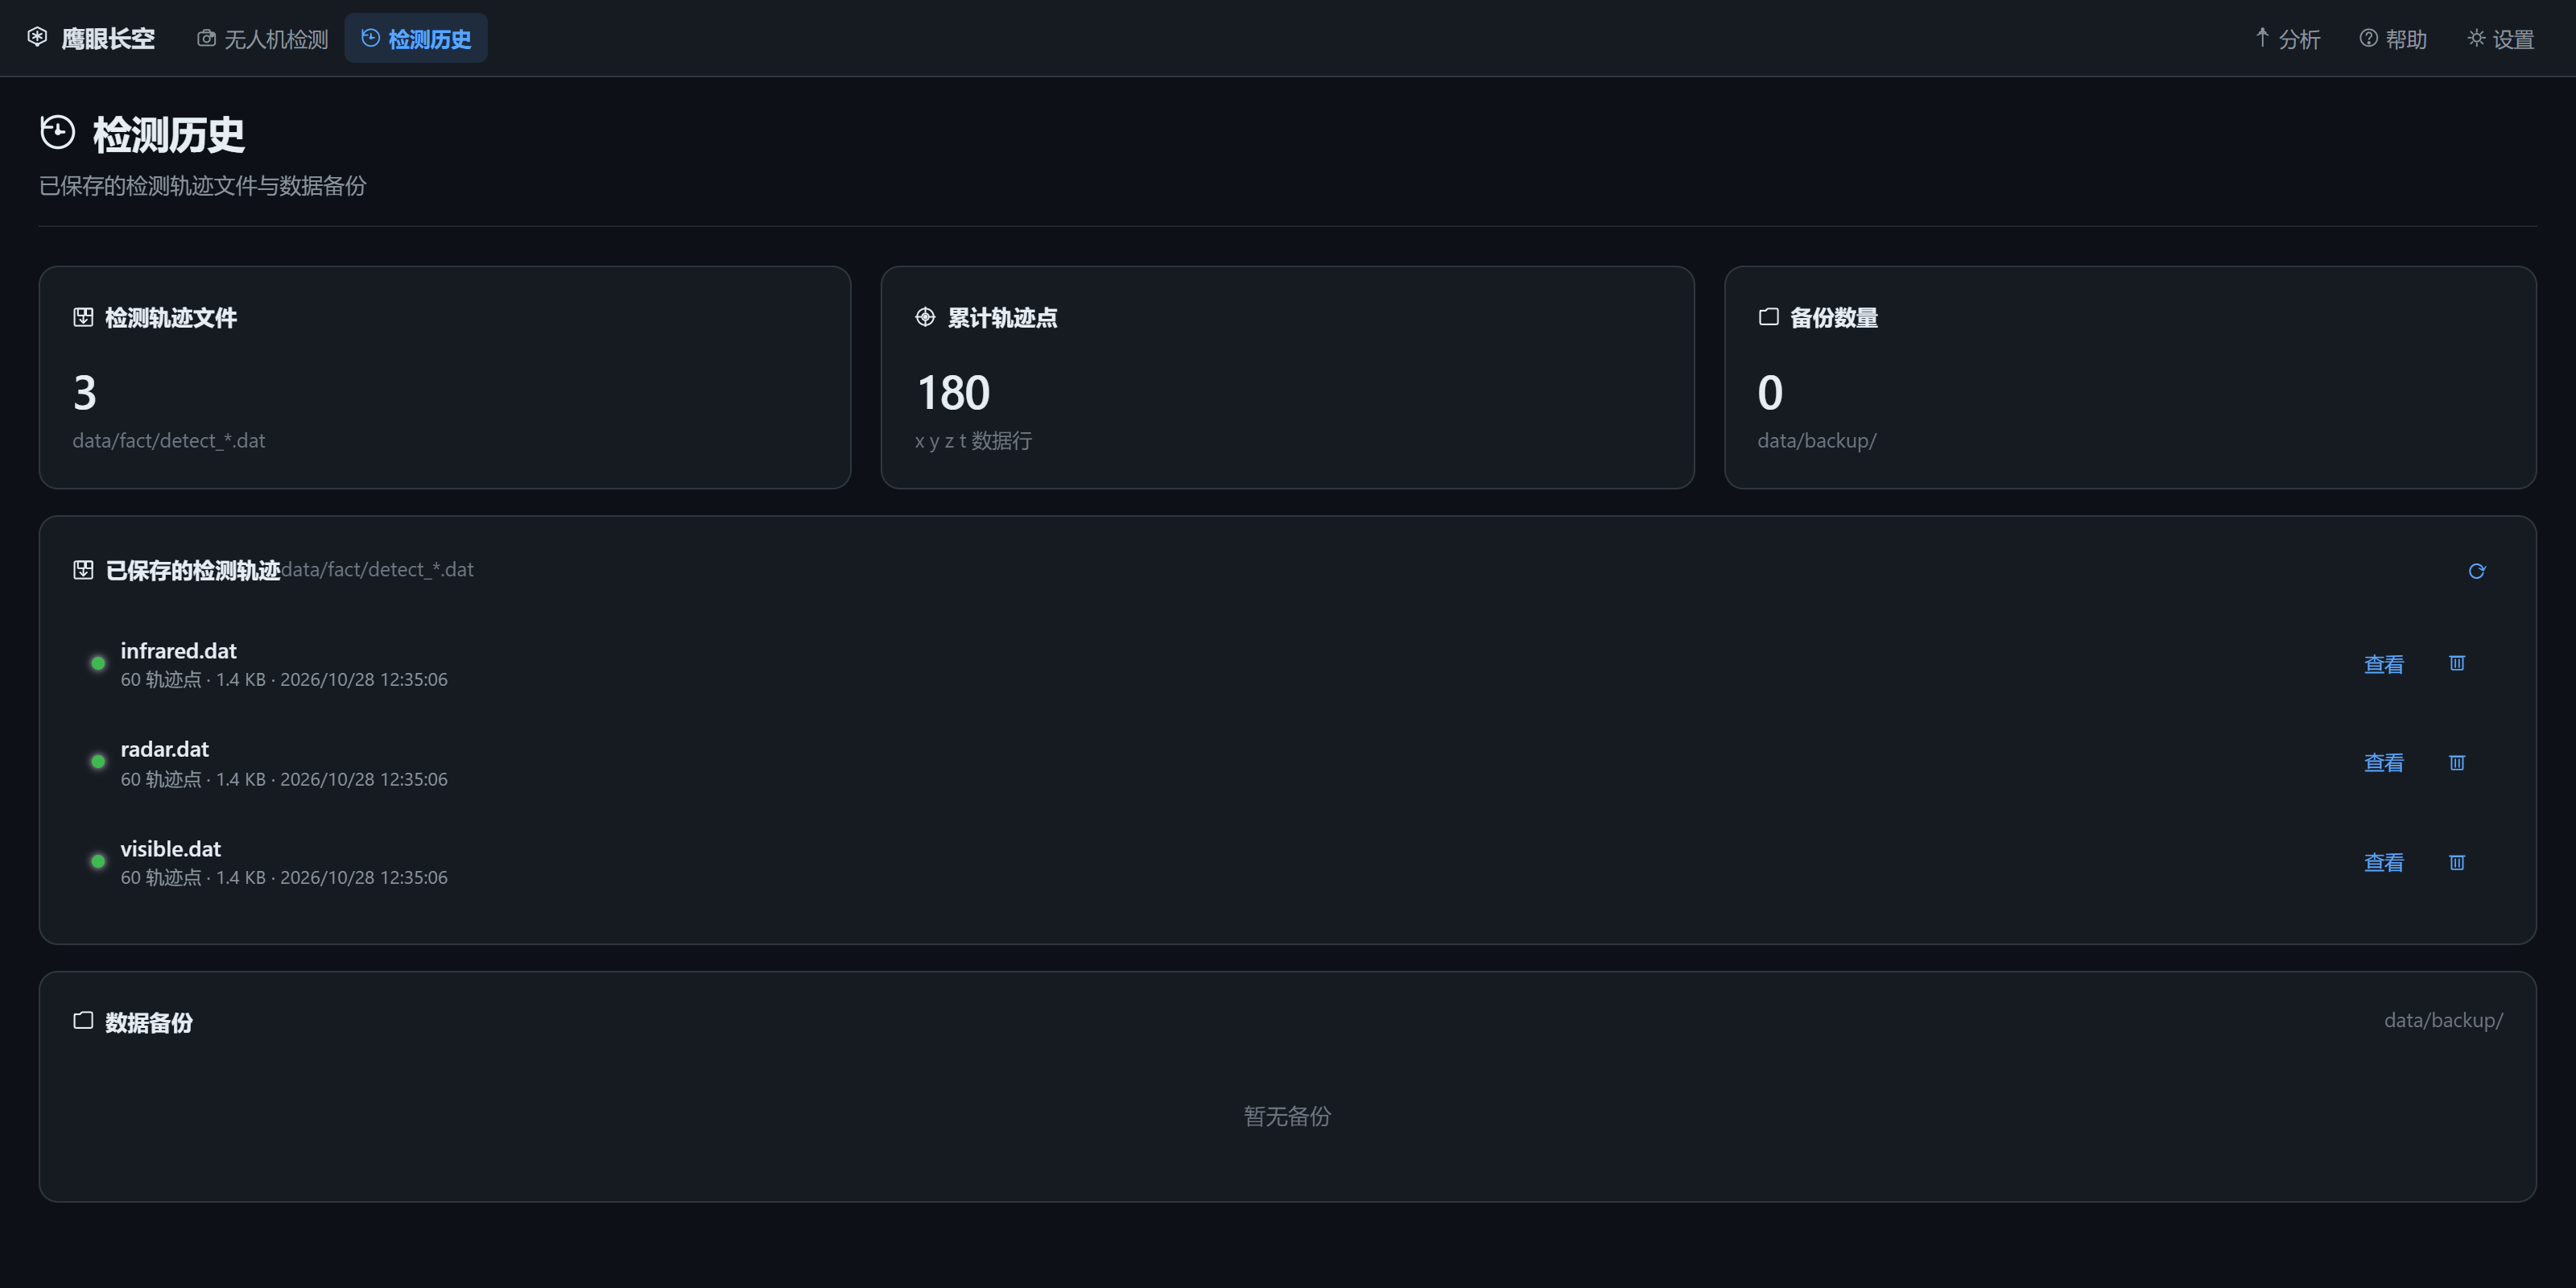
\includegraphics[width=\linewidth]{figures/ui/detect_history.png}};
\begin{scope}[x={(im.south east)},y={(im.north west)}]
  \hotspot{1}{0.300}{0.730}
  \hotspot{2}{0.945}{0.600}
  \hotspot{3}{0.945}{0.200}
\end{scope}
\end{tikzpicture}
\caption{检测历史页操作区域：\cn{1}~统计卡片\quad \cn{2}~轨迹文件列表\quad \cn{3}~备份列表}
\label{fig:use_detect_history}
\end{figure}

\begin{enumerate}
  \item \term{统计卡片（\cn{1}）}：轨迹文件数、累计轨迹点与备份数量。
  \item \term{轨迹文件列表（\cn{2}）}：显示平台名、点数、大小与修改时间，可查看或删除；删除前请确认已备份。
  \item \term{备份列表（\cn{3}）}：快照的时间、标签、文件数与点数；恢复操作在 5000 端口数据页完成，两个模块共用同一备份目录。
\end{enumerate}

\subsection{典型使用流程}

把常用操作串成三条流程，便于新用户按图索骥（图~\ref{fig:use_flow_view}--\ref{fig:use_flow_detect}）。

\begin{figure}[H]
\centering
\begin{tikzpicture}[node distance=6mm]
\node[term] (s) {启动软件};
\node[proc, below=6mm of s, text width=54mm] (p1) {打开总览页（5000）};
\node[proc, below=6mm of p1, text width=54mm] (p2) {按需隐藏/显示平台};
\node[proc, below=6mm of p2, text width=54mm] (p3) {旋转、缩放、平移视角};
\node[proc, below=6mm of p3, text width=54mm] (p4) {播放动画，悬停读点};
\node[term, below=6mm of p4] (e) {形成态势判断};
\foreach \a/\b in {s/p1,p1/p2,p2/p3,p3/p4,p4/e} \draw[arr] (\a) -- (\b);
\end{tikzpicture}
\caption{流程一：快速查看多平台态势}
\label{fig:use_flow_view}
\end{figure}

\begin{figure}[H]
\centering
\begin{tikzpicture}[node distance=6mm]
\node[term] (s) {总览页};
\node[proc, below=6mm of s, text width=58mm] (p1) {进入预测页，选平台与参数并预测};
\node[deci, below=7mm of p1] (d1) {预测成功};
\node[proc, below left=9mm and 6mm of d1, text width=46mm] (p2) {分析页看曲线与捕捉时机};
\node[proc, below right=9mm and 6mm of d1, text width=40mm] (p3) {调整点数/步长重试};
\node[proc, below=6mm of p2, text width=46mm] (p4) {AI 策略页生成建议};
\node[term, below=6mm of p4] (e) {形成处置建议};
\draw[arr] (s) -- (p1); \draw[arr] (p1) -- (d1);
\draw[arr] (d1.west) -| node[lbl, above, pos=0.7]{是} (p2.north);
\draw[arr] (d1.east) -| node[lbl, above, pos=0.7]{否} (p3.north);
\draw[arr] (p3.south) |- (p1.east);
\draw[arr] (p2) -- (p4); \draw[arr] (p4) -- (e);
\end{tikzpicture}
\caption{流程二：预测—分析—AI 策略}
\label{fig:use_flow_analyze}
\end{figure}

\begin{figure}[H]
\centering
\begin{tikzpicture}[node distance=6mm]
\node[term] (s) {检测工作台};
\node[proc, below=6mm of s, text width=62mm] (p1) {上传左右目视频或填写流地址};
\node[proc, below=6mm of p1, text width=62mm] (p2) {选平台，调置信度与抽帧间隔};
\node[proc, below=6mm of p2, text width=62mm] (p3) {开始检测，观察预览与进度};
\node[proc, below=6mm of p3, text width=62mm] (p4) {保存结果（或开启自动保存）};
\node[proc, below=6mm of p4, text width=62mm] (p5) {总览页刷新查看新轨迹};
\node[term, below=6mm of p5] (e) {轨迹可供预测与分析};
\foreach \a/\b in {s/p1,p1/p2,p2/p3,p3/p4,p4/p5,p5/e} \draw[arr] (\a) -- (\b);
\end{tikzpicture}
\caption{流程三：从视频检测到轨迹入库}
\label{fig:use_flow_detect}
\end{figure}

\subsection{常见问题速查}

\begin{table}[H]
\centering
\caption{常见问题与处理办法}
\label{tab:use_faq}
\small
\begin{tabularx}{\linewidth}{@{}>{\heiti}p{4.0cm}>{\raggedright\arraybackslash}X@{}}
\toprule
现象 & 原因与处理 \\
\midrule
提示端口被占用 & 程序会自动清理；仍失败时用 \code{netstat -ano | findstr :5000} 找到进程并结束 \\
页面空白或样式缺失 & 浏览器强制刷新（Ctrl+F5）；确认通过 5000/5001 地址进入 \\
桌面窗口打不开 & 缺少 WebView2 运行时；安装后重试，或改用 \code{--headless} 模式 \\
总览页没有轨迹 & \file{data/fact/} 无数据；到数据页点“更新全部数据”，或用检测模块生成 \\
分析页没有捕捉卡片 & 尚未预测；先到预测页执行一次预测 \\
预测段是一条直线 & 当前为线性外推兜底，属正常现象 \\
AI 策略报错 & 检查 \code{ai} 段配置与网络连通性 \\
检测没有检测框 & 类别不匹配或置信度偏高；调低置信度、核对 \code{target_classes} \\
检测速度慢 & 无 GPU 时单帧约 1.5 s；增大抽帧间隔或改用 CUDA 版 PyTorch \\
上传文件被拒 & 文件需为每行 \code{x y z t} 的文本，空格分隔、四列齐全 \\
配置损坏无法启动 & 删除 \file{config.json}，重启后按模板自动重建 \\
\bottomrule
\end{tabularx}
\end{table}
